\documentclass[11pt]{article}

\usepackage[margin=1in]{geometry}
\usepackage{tikz}
\usetikzlibrary{patterns}
\usepackage{amsmath, amssymb}
\usepackage{graphicx}
\graphicspath{{./}{assets/}}
\usepackage{float}
\usepackage{hyperref}
\usepackage{booktabs}
\usepackage{siunitx}
\usepackage{caption}
\usepackage{subcaption}
\usepackage{needspace}
\usepackage{longtable}
\usepackage{tabularx}
\usepackage{microtype}

\setlength{\parindent}{0pt}
\setlength{\parskip}{0.7em}

\title{Paesano: Holonomic Autonomous Mobile Robotics Platform\\
\large Architecture, Estimation, and Control}
\author{Joseph Marra}
\date{\today}

\begin{document}

\maketitle

\begin{abstract}
\noindent Paesano is a holonomic indoor mobile robotics platform designed around a Raspberry Pi 5 for high-level autonomy processes and a Raspberry Pi Pico-based low-level motor-control module. The final system integrates wheel odometry, IMU fusion through an Extended Kalman Filter, Monte Carlo Localization with a likelihood-field model using LiDAR data, a custom inflated clearance-aware cost map, planning with A$^{*}$ on this cost map, spline-based trajectory generation, and Linear Quadratic Regulator path tracking. A custom iOS mobile application provides teleoperation, mode management, live map and localization visualization, and navigation control. This is done through an HTTP and WebSocket bridge running on the robot. Two experiments were conducted to evaluate Paesano. The first measured low-level velocity and stop behavior across forward, lateral, and rotational commands. The second evaluated full-stack trajectory-following performance. Across nine navigation trials, the system achieved a mean cross-track error of \SI{0.0088}{m} and a mean final position error of \SI{0.0059}{m} in the LiDAR-localized map frame, along with a 100\% route-completion success rate. The complete listed bill of materials totals approximately \$644.04.
\end{abstract}

\begin{figure}[htbp]
    \centering
    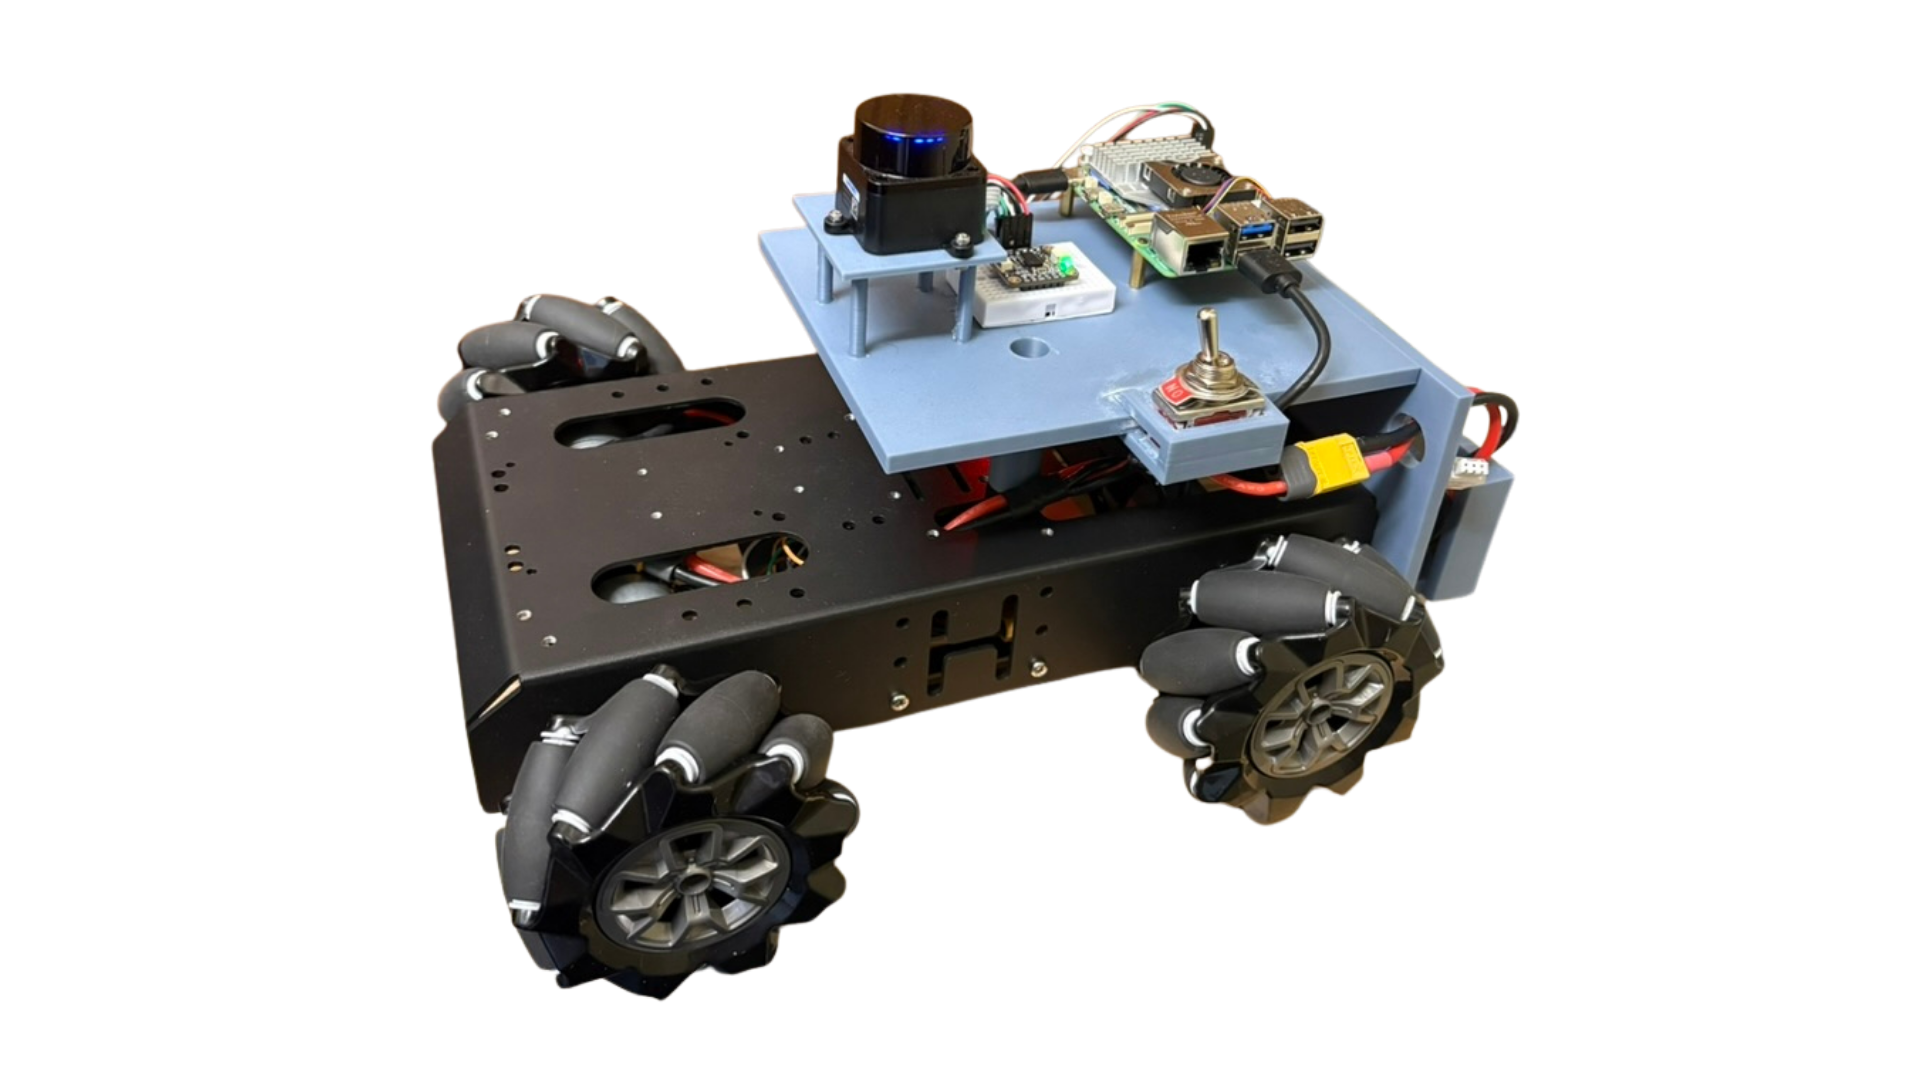
\includegraphics[width=0.80\textwidth]{bot.png}
    \caption{Paesano assembled hardware platform.}
    \label{fig:paesano-platform}
\end{figure}
\newpage
\tableofcontents
\newpage

\section{Hardware Architecture}
\subsection{Parts List}
\noindent Prices shown below are approximate and may fluctuate over time based on
vendor availability, shipping, and market conditions.
\noindent Total estimated cost of listed components: \$644.04.

\begin{longtable}{p{0.72\textwidth} p{0.20\textwidth}}
\caption{Bill of materials for the Paesano platform.}\label{tab:bom}\\
\toprule
Part & Cost (USD) \\
\midrule
\endfirsthead
\toprule
Part & Cost (USD) \\
\midrule
\endhead
HiWonder Chassis Kit & \$185.00 (approx.) \\
PCB Kit (prototype PCB, headers, and assembly materials) & \$9.99 \\
Raspberry Pi 5 w/ Power Supply and Active Cooler & \$162.99 \\
LD19 LiDAR & \$74.90 \\
Buck Converter (USB-C 5V 5A) & \$9.99 \\
22AWG Arduino Wires (Assorted) & \$6.98 \\
Power Switch & \$7.99 \\
Standoffs & \$7.99 \\
Heat Shrink & \$7.99 \\
5V Buck Converter & \$8.99 \\
5200mAh LiPo Battery & \$35.99 \\
LiPo Charger & \$39.98 \\
Raspberry Pi Pico (3x) & \$14.59 \\
XT60 Connectors & \$10.99 \\
XT60 1-to-2 Splitter & \$12.88 \\
BNO085 & \$24.95 \\
Motor Drivers & \$9.90 \\
Wago Connectors & \$11.95 \\
\bottomrule
\end{longtable}

\subsubsection{Additional Required Tools}
\begin{itemize}
    \item Assorted screwdrivers
    \item Soldering iron
    \item Multimeter
    \item Access to a 3D printer
\end{itemize}

\subsection{System Overview}
The system was designed around a clear separation between high-level autonomy and low-level motor control. This allows the high-level autonomy module to run estimation, planning, navigation, and operator-facing services without also carrying the timing burden of direct motor actuation.

The high-level compute module, a Raspberry Pi 5 running Ubuntu 24.04 LTS, handles state estimation, navigation, trajectory following, and communication with the mobile application. The motor control module, built around a Raspberry Pi Pico and two TB6612 motor drivers, manages deterministic low-level control of the drivetrain. This separation improves modularity, simplifies debugging, and makes future hardware or firmware changes less disruptive to the rest of the platform.

Figure~\ref{fig:system-architecture} shows the resulting system architecture and the primary flow of power and information between components.

\begin{figure}[htbp]
    \centering
    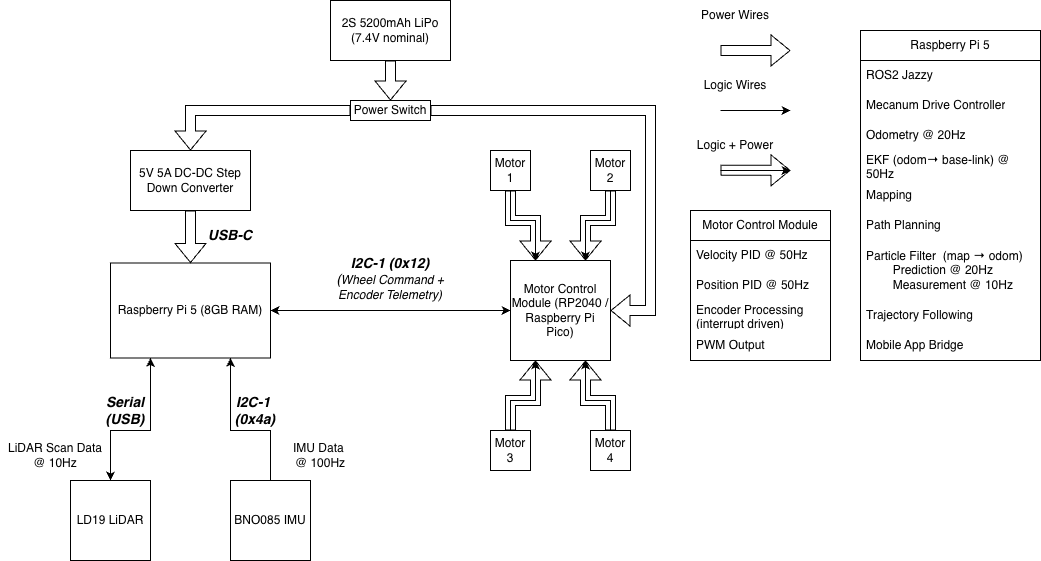
\includegraphics[width=\textwidth]{System Architecture.png}
    \caption{System architecture overview.}
    \label{fig:system-architecture}
\end{figure}

\subsection{Power Architecture}
The robot is powered by a \SI{7.4}{V} nominal 2S \SI{5200}{mAh} LiPo battery, acting as the "heart" of the robot. This battery directly powers the entire system and was selected for its high energy density and ability to provide the necessary current for all components, especially the motor drivers.
A dedicated DC-DC converter is used to step down the voltage and amperage to appropriate levels for the Raspberry Pi 5,
ensuring stable power delivery and preventing brownouts. The motors themselves are powered directly from the \SI{7.4}{V} supply, since they are designed to operate at this voltage.
The Pico is powered from a regulated \SI{5}{V} rail within the motor control module.

\Needspace{0.7\textheight}
\subsection{Motor Control Stack}
The HiWonder chassis originally came with its own motor control module and PID controller. However, the available hardware was limited and the firmware was not practical to customize for this project. A dedicated motor control module was therefore designed around the Pico and two TB6612 dual motor drivers.

This motor control module performs closed-loop control of the four DC motors at a fixed update rate of \SI{50}{Hz}. Offloading these tasks to a microcontroller keeps the low-level loop deterministic and allows the Raspberry Pi 5 to reserve its compute resources for higher-level autonomy tasks. Figure~\ref{fig:motor-control-module} shows the schematic of this subsystem.
\begin{figure}[H]
    \centering
    \includegraphics[width=0.95\textwidth]{motor_control_module.pdf}
    \caption{Motor Control Module.}
    \label{fig:motor-control-module}
\end{figure}

\subsection{Sensor Suite}
The robot uses a combination of wheel encoders, IMU, and LiDAR for perception and state estimation. A BNO085 IMU provides orientation 
and angular velocity measurements at approximately \SI{100}{Hz}. IMU data is fused with wheel odometry calculated using wheel encoders in an Extended
Kalman Filter to produce a smooth local state estimate. An LD19 2D LiDAR sensor provides planar range 
measurements which are used for mapping and localization. The scan data is produced at approximately \SI{10}{Hz}.
\begin{itemize}
    \item IMU Datasheet/Documentation: \url{https://www.adafruit.com/product/4754}
    \item LiDAR Datasheet/Documentation: \url{https://wiki.youyeetoo.com/en/Lidar/D300}
\end{itemize}

\subsection{Mechanical Design}
The chassis from HiWonder provided motors with encoders and a main chassis frame. However, it did not come with any intuitive way to 
mount the various sensors, batteries, and other processing units. To address this, several custom parts were designed to integrate these systems
into the platform. These parts were designed using OnShape and then printed on a Bambu Lab X1 Carbon in PLA.

\begin{figure}[htbp]
    \centering
    \begin{subfigure}[b]{0.40\textwidth}
        \centering
        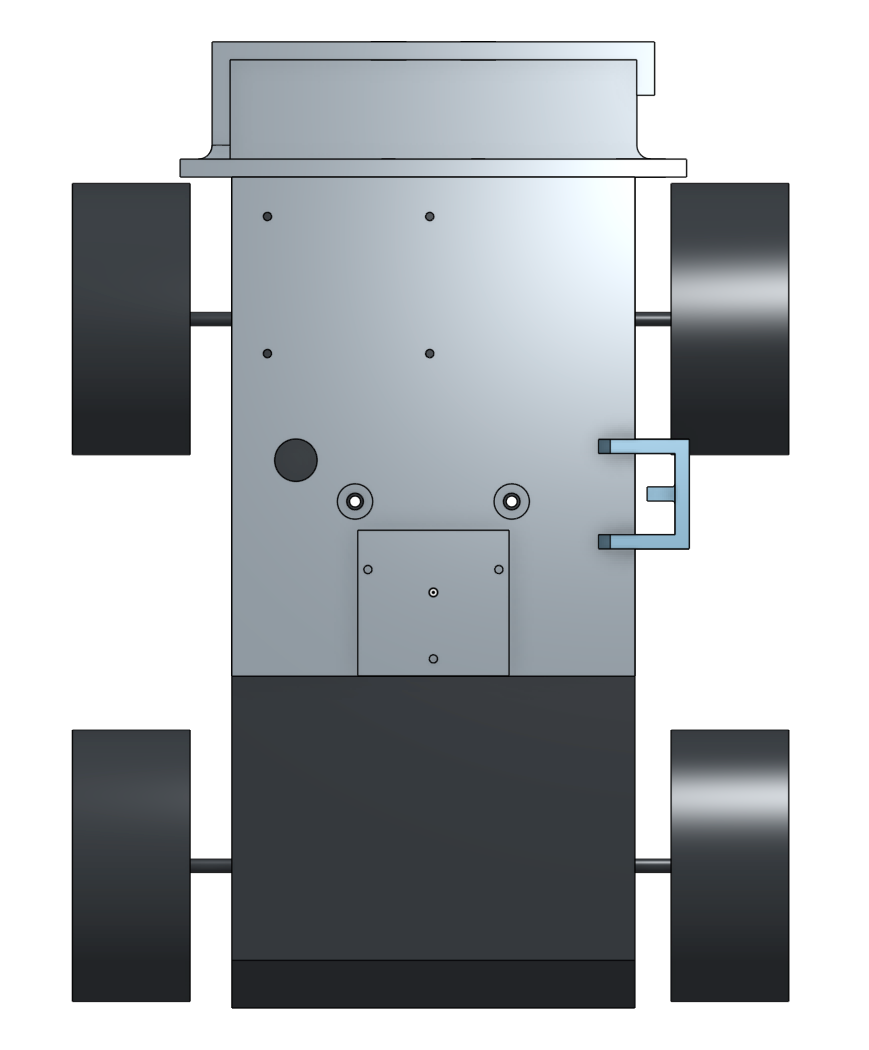
\includegraphics[width=\textwidth]{cad_0.png}
        \caption{CAD Bird's Eye View}
        \label{fig:cad-0}
    \end{subfigure}
    \hfill
    \begin{subfigure}[b]{0.40\textwidth}
        \centering
        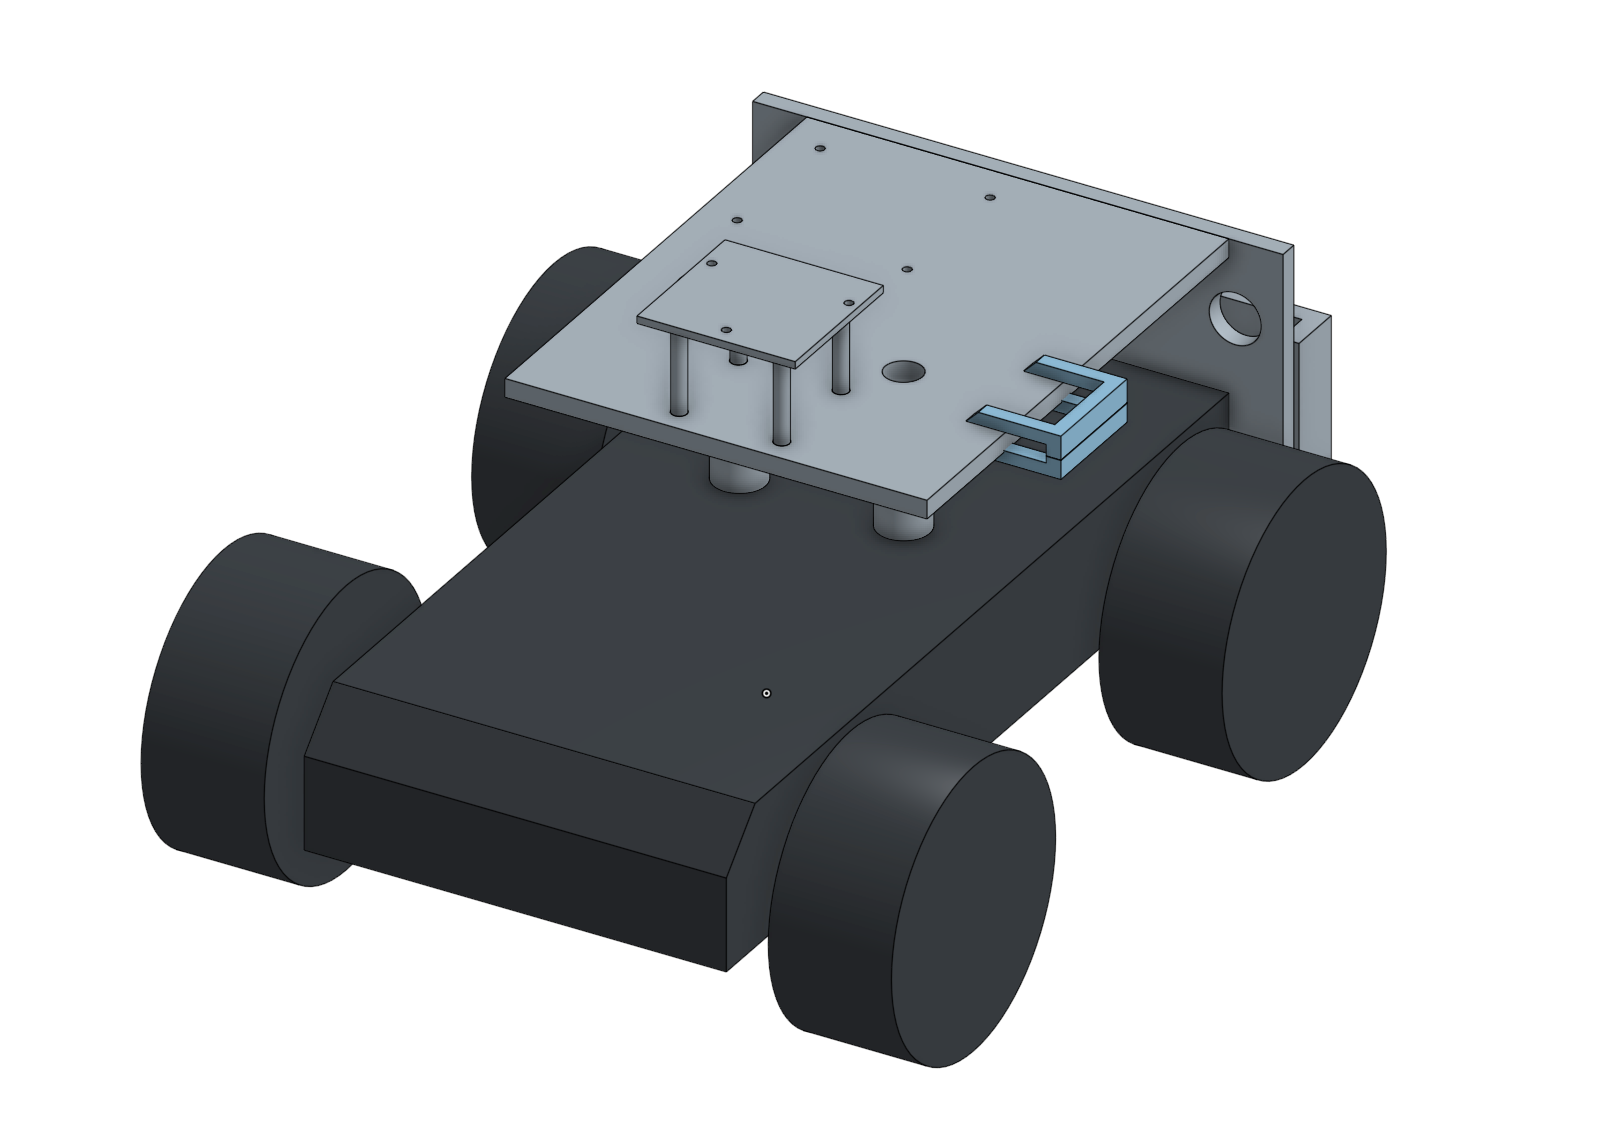
\includegraphics[width=\textwidth]{cad_1.png}
        \caption{CAD Isometric View}
        \label{fig:cad-1}
    \end{subfigure}
    \caption{Mechanical CAD models of the platform and custom mounts.}
    \label{fig:mechanical-cad}
\end{figure}

\noindent The parts in gray and in blue are the ones that were custom designed and printed. The part in black is a model of the HiWonder chassis
to make designing the custom parts easier. The parts in gray include a stand for the LiDAR, a mounting plate for the Raspberry Pi 5 and IMU,
and a battery compartment in the back. The blue part is a power switch holder, and once printed it is to be super glued
onto the gray mounting plate wherever desired.

\subsection{Design Philosophy}
The platform was designed around modularity, simplicity, expandability, accessibility, and cost effectiveness. 
\begin{itemize}
    \item Modularity: low-level motor control is isolated from the autonomy stack, and the major ROS 2 subsystems communicate through explicit and standardized interfaces. This made it practical to debug and revise one layer without destabilizing the rest of the robot.
    \item Simplicity: The design prioritizes straightforward implementation and maintenance, ensuring that the robot can be easily understood and modified by developers.
    \item Expandability: The platform is designed to accommodate future enhancements and modifications, with spare compute headroom, open mounting space, and software abstraction layers preserved for future sensors or estimation methods.
    \item Accessibility: The design ensures that components are easily accessible for maintenance and upgrades, without requiring too much disassembly.
    \item Cost Effectiveness: Component selection was influenced by the need to balance performance with cost, ensuring that the platform remains practical and affordable while meeting its functional requirements.
\end{itemize}

\section{Firmware}
All firmware for this project was written in C++ for compatibility with the RP2040 microcontroller on the Pico and for predictable runtime performance. The firmware is responsible for real-time motor control, encoder processing, and communication with the Raspberry Pi 5. Because motor control requires consistent timing and low latency, this layer operates independently of the higher-level ROS 2 stack.
\subsection{Communication Protocol}
Communication between the Raspberry Pi 5 and the Pico is implemented over I\textsuperscript{2}C, with the Raspberry Pi 5 acting as the bus master and the Pico configured as an I\textsuperscript{2}C slave at address \texttt{0x12}. 
The Raspberry Pi 5 reads and writes register-mapped data to exchange control commands and telemetry.

\begin{table}[H]
    \centering
    \caption{I\textsuperscript{2}C register map between the Raspberry Pi 5 and Pico.}
    \label{tab:i2c-register-map}
    \begin{tabularx}{\textwidth}{@{}p{0.20\textwidth}p{0.21\textwidth}p{0.14\textwidth}X@{}}
        \toprule
        Name & Address/Register & Pico Access & Purpose \\
        \midrule
        \texttt{I2C\_ADDR} & \texttt{0x12} & N/A & 7-bit I\textsuperscript{2}C slave address for the Pico. \\
        \texttt{REG\_MOTOR\_SPEEDS} & \texttt{51} & Read & Sets wheel/motor speed targets. \\
        \texttt{REG\_ENCODERS} & \texttt{60} & Write & Readback register for encoder counts. \\
        \texttt{REG\_PID\_GAINS} & \texttt{70} & Read & Configuration register for PID gain parameters. \\
        \bottomrule
    \end{tabularx}
\end{table}
\noindent In Table~\ref{tab:i2c-register-map}, the \textit{Pico Access} column is written from the Pico's perspective as the I\textsuperscript{2}C slave. A register marked \textit{Read} is read by the Pico when the Raspberry Pi writes into it, while a register marked \textit{Write} is written by the Pico so the Raspberry Pi can read the resulting telemetry.

\subsection{Control Loop Architecture}
The main control loop of the firmware runs every \SI{0.02}{s}, or at \SI{50}{Hz}. Encoder measurements are used to 
estimate wheel velocities, which are fed into a cascaded control system. There are two possible modes: drive and hold.

In drive mode, the robot moves at the commanded velocity using a velocity PID with 
feedforward compensation. In hold mode (after the robot has been commanded to stop), a position controller 
generates velocity targets based on the error between the current position and the position at the time the robot was 
commanded to stop so it remains in place. These targets are then tracked by the velocity PID controller. The resulting PWM signals from either mode are sent to the 
TB6612 motor drivers. 
\begin{figure}[htbp]
    \centering 
    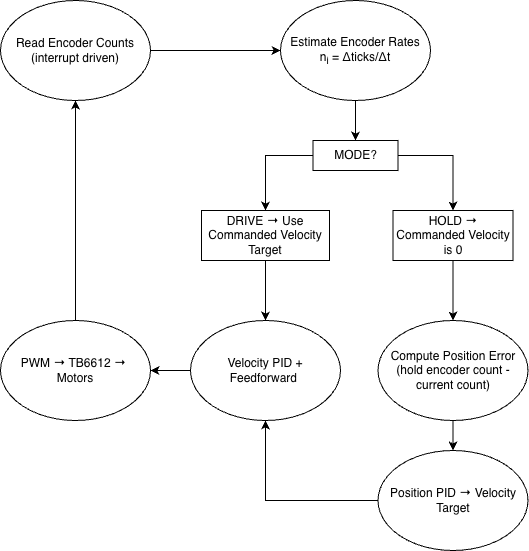
\includegraphics[width=0.40\textwidth]{controltick.png}
    \caption{Control loop timing diagram.}
    \label{fig:control-loop-timing}
\end{figure}

\subsection{Motor Control Algorithms}
As described above, motor velocity and position control is done using separate velocity and position PID controllers. Both controllers' integral term is 
capped when the control output saturates. 
\subsubsection{Velocity PID Control}
\begin{equation*}
e_v(t) = v_{\mathrm{ref}}(t) - v(t)
\end{equation*}
\begin{equation*}
u_v(t) = K_{p,v} e_v(t) + K_{i,v}\operatorname{clip}\!\left(\int_0^t e_v(\tau)\,d\tau,\,-I_{\max,v},\,I_{\max,v}\right) + K_{d,v}\frac{d e_v(t)}{dt} + K_{\mathrm{ff}}\,v_{\mathrm{ref}}(t)
\end{equation*}
\subsubsection{Position PID Control}
\begin{equation*}
e_p(t) = p_{\mathrm{ref}}(t) - p(t)
\end{equation*}
\begin{equation*}
v_{\mathrm{ref}}(t) = K_{p,p} e_p(t) + K_{i,p}\operatorname{clip}\!\left(\int_0^t e_p(\tau)\,d\tau,\,-I_{\max,p},\,I_{\max,p}\right) + K_{d,p}\frac{d e_p(t)}{dt}
\end{equation*}
\noindent In practice, the velocity controller handles normal motion tracking while the position controller is only engaged after a stop command. This arrangement keeps the robot responsive during motion and reduces residual drift once the commanded velocity returns to zero.
\section{Software Architecture}
The software runs on the Raspberry Pi 5 using ROS 2 Jazzy on Ubuntu 24.04 LTS. The stack is organized as a set of nodes for sensing, estimation, planning, control, and user interaction, which keeps the major subsystems modular and connected through topic, service, and action interfaces.

In both operating modes, bringup launches the IMU driver, the LD19 LiDAR driver, the mecanum drive controller, the odometry node, the IMU covariance republisher, and the EKF. Mapping mode additionally launches \texttt{slam\_toolbox}, while localization mode launches the particle filter, the A$^*$ action server, and the LQR trajectory follower. The mobile bridge runs as both a ROS 2 node and a FastAPI/Uvicorn server, and switches modes by restarting bringup with the \texttt{localization\_mode} launch argument set appropriately.

Sensor data such as wheel encoder counts, IMU readings, and LiDAR scans are published on dedicated topics and fused into a consistent state estimate. In mapping mode, the bridge publishes teleoperation commands directly to \texttt{/cmd\_vel}. In localization mode, \texttt{/cmd\_vel} may instead come from either teleoperation or the LQR tracker during autonomous path following.

\begin{figure}[H]
    \centering
    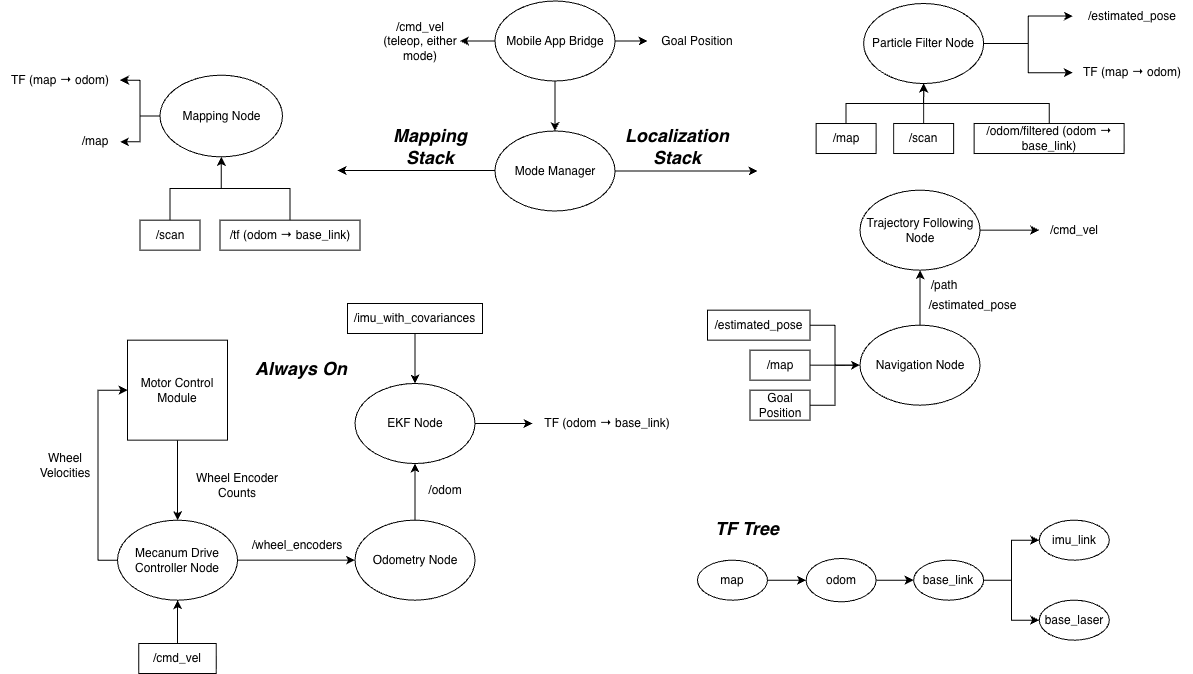
\includegraphics[width=0.99\textwidth]{softarch.png}
    \caption{Software architecture overview.}
    \label{fig:software-architecture}
\end{figure}

The TF frame tree defines the relationships between the robot base (\texttt{base\_link}), odometry frame (\texttt{odom}), map frame (\texttt{map}), and onboard sensors (\texttt{base\_laser}, \texttt{imu\_link}). These transforms are used by localization, navigation, and control nodes so that pose estimates and commands remain consistent across the full software stack.

\section{Kinematics}
To achieve holonomic motion, the robot uses a mecanum wheel drivetrain. Alternative systems such as swerve drive offer superior traction, efficiency, and 
high-speed performance, but they also require additional steering actuators and more complex mechanical control systems. For this project, 
that increased complexity was not justifiable on a time or budget basis. 

Mecanum drive was chosen because it provides omnidirectional movement using only four drive motors, yielding a mechanically simple but fully holonomic platform. A differential-drive robot would have been simpler, but it would not have supported lateral motion or the broader kinematic and control challenges that motivated the project.
\noindent In the final real-hardware implementation, the drivetrain no longer uses a
normalized wheel-mixing approximation. Instead, the high-level motor controller
interprets \texttt{/cmd\_vel} in SI units and applies geometry-based inverse
kinematics using the measured platform dimensions:
\[
r = \SI{0.0485}{m}, \qquad
L = \SI{0.212}{m}, \qquad
W = \SI{0.194}{m}, \qquad
R = \frac{L+W}{2} = \SI{0.203}{m}
\]
\noindent For a commanded body-frame twist
\[
\mathbf{u} =
\begin{bmatrix}
v_x\\
v_y\\
\omega
\end{bmatrix},
\]
the wheel rim linear velocities are computed as
\begin{equation*}
\begin{bmatrix}
v_{\mathrm{FL}} \\
v_{\mathrm{FR}} \\
v_{\mathrm{BL}} \\
v_{\mathrm{BR}}
\end{bmatrix}
=
\begin{bmatrix}
1 & -1 & -R \\
1 & 1 & R \\
1 & 1 & -R \\
1 & -1 & R
\end{bmatrix}
\begin{bmatrix}
v_x \\
v_y \\
\omega
\end{bmatrix}
\end{equation*}
\noindent where $v_x$ and $v_y$ are the commanded translational velocities in
\si{m/s} and $\omega$ is the commanded yaw rate in \si{rad/s}.

\noindent These wheel rim velocities are then converted into encoder tick-rate
targets using the known encoder resolution of $N_{enc}=2882$ ticks per
revolution. Since the linear distance traveled per encoder tick is
\[
d_{\mathrm{tick}} = \frac{2\pi r}{N_{enc}},
\]
the target wheel tick rates become
\[
\dot{n}_i = \frac{v_i}{d_{\mathrm{tick}}}
=
v_i \frac{N_{enc}}{2\pi r}.
\]

\noindent To keep the commanded motion within the measured hardware envelope, the
body-frame command is first clamped to
\[
\sqrt{v_x^2 + v_y^2} \le \SI{0.35}{m/s},
\qquad
|\omega| \le \SI{1.5}{rad/s}.
\]
After inverse kinematics, if any wheel target exceeds the configured maximum of
\SI{3500}{ticks/s}, all four wheel targets are scaled by the same factor so that
the requested motion direction is preserved while remaining inside the actuator
limits. The final tick-rate targets are then normalized to the Pico's signed
\texttt{int8} command range before being sent over I\textsuperscript{2}C.
\section{Odometry}
Wheel odometry provides a local estimate of robot motion by integrating measured wheel velocities over time. This estimate is subject to
drift due to wheel slip, friction, noise, and other factors, but it provides a high-frequency state estimate that becomes useful for localization later on.
It is calculated using encoder measurements from each of the four drive motors. Each one provides incremental encoder counts
(approximately 2882 per revolution) which are first converted to encoder tick rates and then to wheel linear speeds. From these measurements the robot body velocity is estimated and then integrated
to produce a pose estimate in the odom frame.

Let $\Delta n_i$ denote the change in encoder ticks for wheel $i$ over a
time interval $\Delta t$. The implementation first computes the encoder tick
rate
\[
\dot{n}_i = \frac{\Delta n_i}{\Delta t}
\]
and then converts it into wheel rim linear speed using the measured distance per
encoder tick
\[
d_{\mathrm{tick}} = \frac{2\pi r}{2882},
\qquad
v_i = \dot{n}_i d_{\mathrm{tick}}.
\]

The robot velocity is then estimated using the mecanum wheel forward kinematics. This matrix maps the individual wheel
velocities to the robot translational velocity and angular velocity:
\begin{equation*}
\begin{bmatrix}
v_{x,\mathrm{body}} \\
v_{y,\mathrm{body}} \\
\omega
\end{bmatrix}
=
\begin{bmatrix}
\frac{1}{4} & \frac{1}{4} & \frac{1}{4} & \frac{1}{4} \\
-\frac{1}{4} & \frac{1}{4} & \frac{1}{4} & -\frac{1}{4} \\
-\frac{1}{4(L+W)} & \frac{1}{4(L+W)} & -\frac{1}{4(L+W)} & \frac{1}{4(L+W)}
\end{bmatrix}
\begin{bmatrix}
v_{\mathrm{FL}} \\
v_{\mathrm{FR}} \\
v_{\mathrm{BL}} \\
v_{\mathrm{BR}}
\end{bmatrix}
\end{equation*}

This body-frame velocity is then rotated into the odom frame using the current heading $\theta$:
\begin{equation*}
\begin{bmatrix}
v_{x,\mathrm{odom}} \\
v_{y,\mathrm{odom}}
\end{bmatrix}
=
\begin{bmatrix}
\cos\theta & -\sin\theta \\
\sin\theta & \cos\theta
\end{bmatrix}
\begin{bmatrix}
v_{x,\mathrm{body}} \\
v_{y,\mathrm{body}}
\end{bmatrix}
\end{equation*}

The robot pose is then updated by integrating this velocity in the odom frame:
\begin{align*}
x_{t+1} &= x_t + v_{x,\mathrm{odom}}\Delta t \\
y_{t+1} &= y_t + v_{y,\mathrm{odom}}\Delta t \\
\theta_{t+1} &= \theta_t + \omega \Delta t
\end{align*}
\noindent The resulting \texttt{/odom} message therefore carries pose in the
\texttt{odom} frame and twist in the \texttt{base\_link} frame. The odometry
node does not publish TF directly; the \texttt{odom} $\to$ \texttt{base\_link}
transform is later produced by the EKF.


\section{State Estimation}
State estimation is split into local (Extended Kalman Filter) and global (Monte Carlo Localization) layers.
The EKF fuses wheel odometry and IMU data to produce a smooth local estimate in the odom frame; however, it is still subject to slip and drift. In the current launch structure, the EKF runs in both mapping and localization modes. Monte Carlo Localization (MCL) is only launched in localization mode, where it uses LiDAR and the known map to correct that drift.
The EKF publishes \texttt{/odom/filtered} together with \texttt{odom} $\to$ \texttt{base\_link}, while MCL publishes \texttt{/estimated\_pose} and \texttt{map} $\to$ \texttt{odom}, giving:
\[
{}^{map}\!T_{base\_link} = {}^{map}\!T_{odom}\,{}^{odom}\!T_{base\_link}
\]

\subsection{Extended Kalman Filter (EKF)}
For this project, the EKF provided by the $robot\_localization$ package was used for simplicity of integration (\url{https://wiki.ros.org/robot_localization}).
\subsubsection{Purpose in the System}
The purpose of the EKF is to generate a high-frequency local state estimate (\(x\)-position, \(y\)-position, \(v_x\), \(v_y\), heading \(\theta\), and heading rate \(\dot{\theta}\)) 
by fusing noisy sensor data from wheel odometry and the IMU, using covariance matrices to represent the relative uncertainty of each measurement. A lightweight preprocessing node first republishes the raw IMU data with the tuned covariance matrices attached, and that covariance-annotated IMU stream is then fused with \texttt{/odom} inside \texttt{robot\_localization}. This local estimate is used as the motion model input for MCL whenever localization mode is active. The underlying prediction/update equations follow the standard $robot\_localization$ implementation. An EKF was chosen because it provides a reasonable balance between estimation accuracy and computational efficiency while handling nonlinearity in the motion model well.
\subsubsection{State Vector}
The EKF estimates a six-dimensional state representing the robot's planar pose and velocity.
\[ \mathbf{x} = [x, y, v_x, v_y, \theta, \dot{\theta}]^T \]
Odometry $x$, $y$, $v_x$, $v_y$, $\theta$, $\dot{\theta}$ and IMU $\theta$, $\dot{\theta}$ were fused to estimate this state. However, since odometry $\theta$ and $\dot{\theta}$ are extremely unreliable,
the covariance matrices were tuned so that odometry primarily informs $x$, $y$, $v_x$, and $v_y$, while the IMU primarily informs $\theta$ and $\dot{\theta}$.
\subsubsection{Covariance Tuning}
The covariance values used for the EKF were informed by experimental odometry measurements. While the experiment was conducted in ideal conditions, the results reveal important relative characteristics of the drivetrain noise.
The experiment shows that forward motion produces the lowest odometry error, while lateral (strafing) motion exhibits significantly higher uncertainty due to the inherent slip characteristics of mecanum wheels. Rotational motion introduces the largest error.
Across the trials, this is the relationship between each covariance:
\[
\sigma_y^2 \approx 10\sigma_x^2, \qquad
\sigma_\theta^2 \approx 10\sigma_y^2
\]

\begin{figure}[htbp]
    \centering
    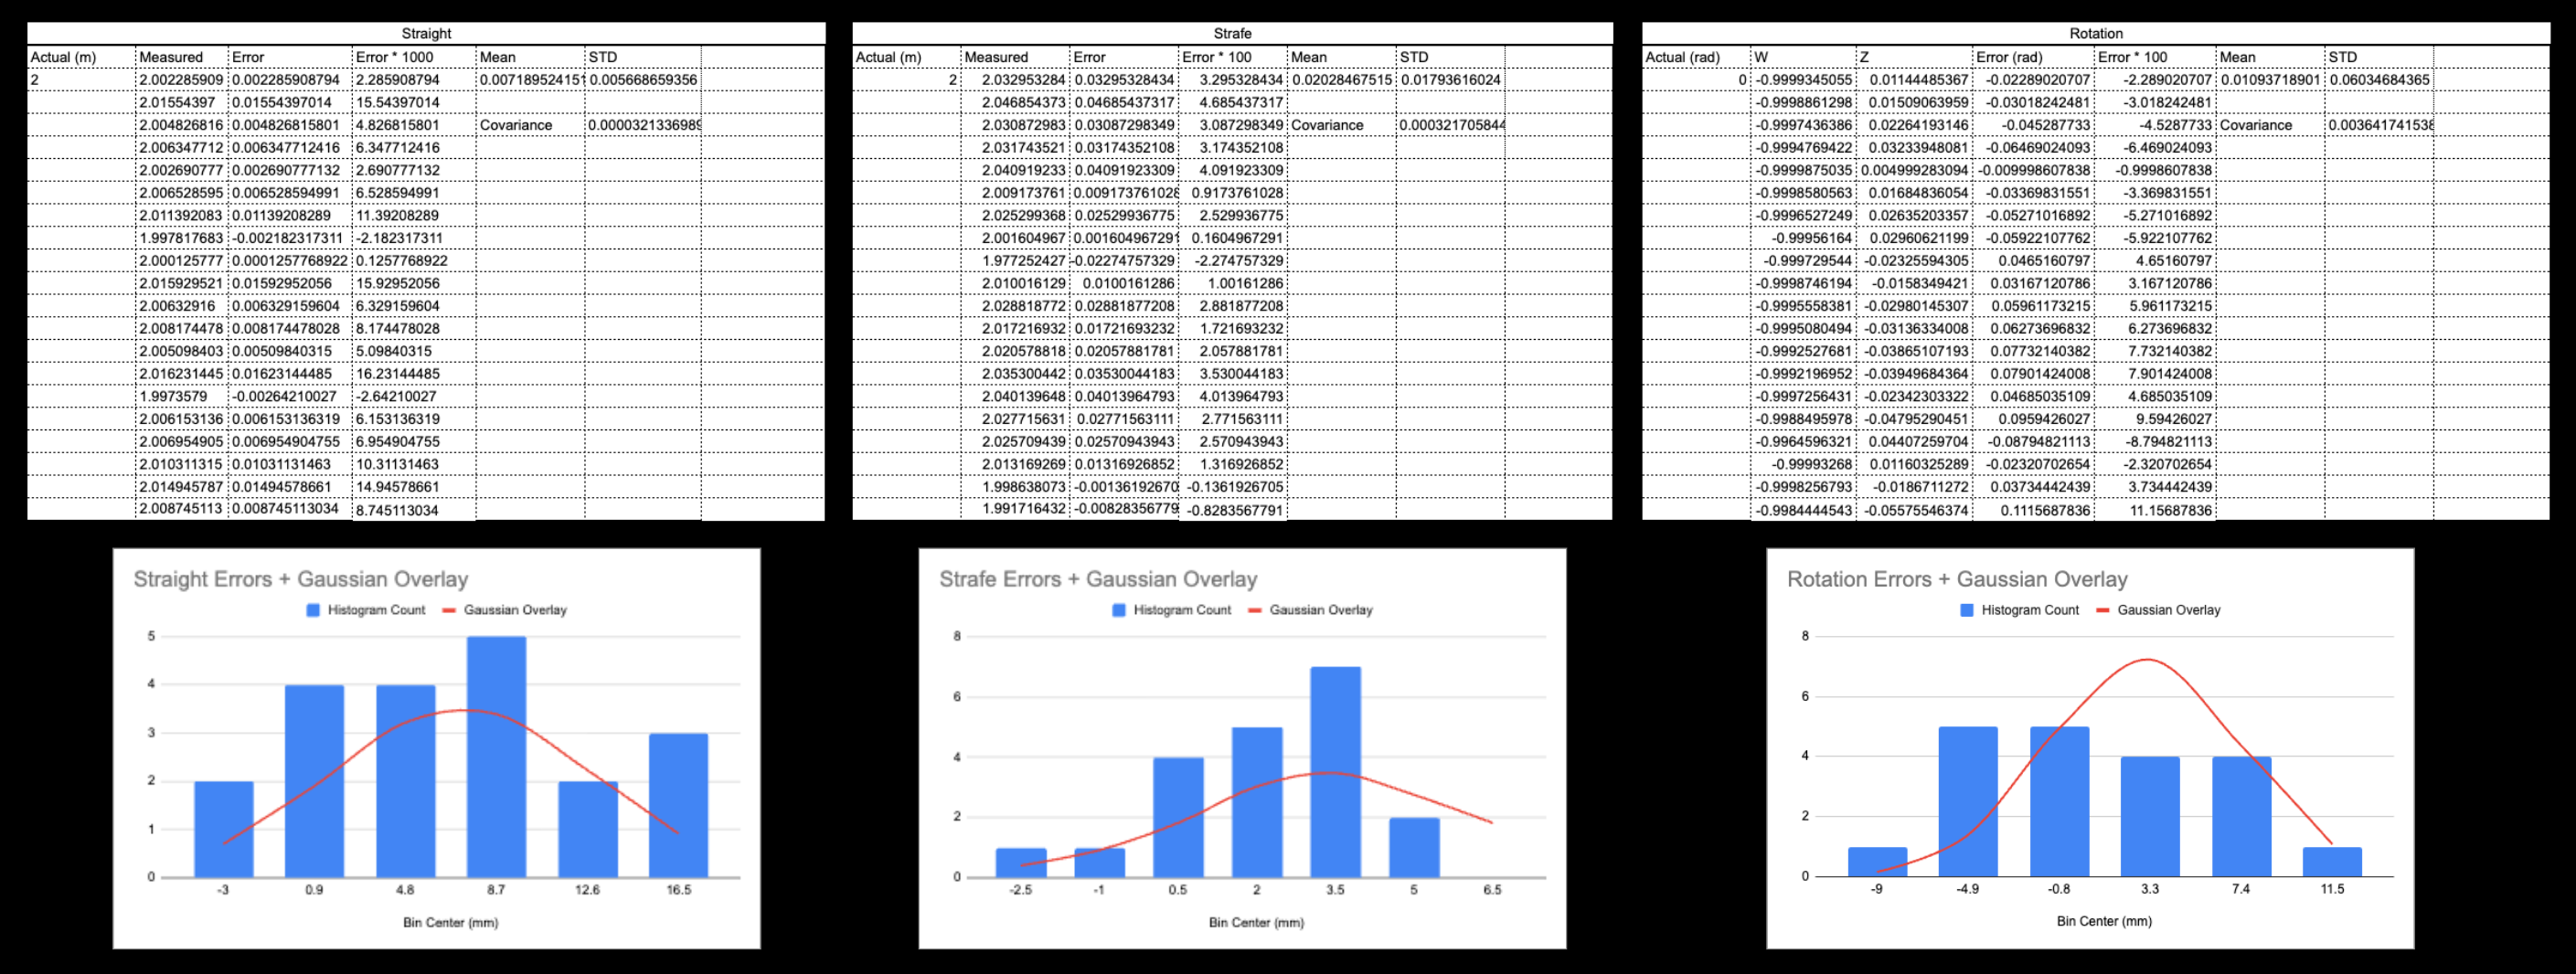
\includegraphics[width=0.98\textwidth]{odom_covariances.png}
    \caption{EKF covariance tuning reference.}
    \label{fig:ekf-covariance-tuning}
\end{figure}

\noindent Because the experiments were conducted under ideal conditions, the resulting covariance values represent optimistic estimates of drivetrain noise. In practice, only two covariance design values had to be tuned: a base covariance and a position-versus-velocity scale factor. The base covariance was assigned to forward motion, while lateral and rotational covariances were set to 10x and 100x that value respectively, following the experimental results. The position-versus-velocity scale factor was set to 0.5, since position is the integral of velocity and velocity generally experiences less noise amplification. IMU covariance was initially estimated from the datasheet noise standard deviation, converted to variance, and then tuned experimentally.

\subsection{Monte Carlo Localization (MCL)}
\subsubsection{Purpose in the System}
Monte Carlo Localization was chosen because it is robust to non-Gaussian uncertainty, multi-modal pose hypotheses, and odometry drift. In this system it acts as the global localization layer on top of the EKF, using LiDAR and the known map to correct accumulated local-frame error. It also pairs naturally with the likelihood-field measurement model and can recover from poor initial pose estimates through reweighting and resampling.

\subsubsection{Bayesian Formulation}
Monte Carlo Localization is derived from the recursive Bayes filter. The belief over the robot state is updated using both the motion model and the sensor model:
\begin{equation}
bel(w_t) =
\eta \, p(z_t \mid w_t)
\int p(w_t \mid w_{t-1}, u_t)\, bel(w_{t-1}) \, dw_{t-1}
\end{equation}
\noindent where
\[
w_t =
\begin{bmatrix}
x_t \\
y_t \\
\theta_t
\end{bmatrix}
\]
\noindent represents the robot pose at time $t$.
\subsubsection{Motion Model}

The motion model uses odometry increments to propagate each particle. First, the odometry displacement is rotated into the robot body frame:
\begin{equation*}
\begin{bmatrix}
\Delta x_{body}\\
\Delta y_{body}
\end{bmatrix}
=
\begin{bmatrix}
\cos(\theta_{odom,t-1}) & \sin(\theta_{odom,t-1})\\
-\sin(\theta_{odom,t-1}) & \cos(\theta_{odom,t-1})
\end{bmatrix}
\begin{bmatrix}
\Delta x_{odom}\\
\Delta y_{odom}
\end{bmatrix}
\end{equation*}
\noindent where \(\theta_{odom,t-1}\) is the odometry heading at time \(t-1\). The body-frame displacement is then rotated into the frame of the particle:
\begin{equation*}
\begin{bmatrix}
\Delta x_{part}\\
\Delta y_{part}
\end{bmatrix}
=
\begin{bmatrix}
\cos(\theta_{part,t-1}) & -\sin(\theta_{part,t-1})\\
\sin(\theta_{part,t-1}) & \cos(\theta_{part,t-1})
\end{bmatrix}
\begin{bmatrix}
\Delta x_{body}\\
\Delta y_{body}
\end{bmatrix}
\end{equation*}
\noindent The particle state is then updated as
\begin{align*}
x_t &= x_{t-1} + \Delta x_{part} \\
y_t &= y_{t-1} + \Delta y_{part} \\
\theta_t &= \theta_{t-1} + \Delta \theta_{odom}
\end{align*}
\noindent To model uncertainty in the propagated particle state, the motion model is represented as a 3D Gaussian with covariance
\[
\Sigma_t =
\begin{bmatrix}
(x_{\text{noise}}\cdot translation)^2 & 0 & 0\\
0 & (y_{\text{noise}}\cdot translation)^2 & 0\\
0 & 0 & (\theta_{\text{noise}}\cdot rotation)^2
\end{bmatrix}.
\]

\noindent Conditioned on the previous particle state and the measured odometry increment, the propagated particle state is modeled as a Gaussian random variable centered at the propagated mean pose:
\begin{equation*}
p(w_t \mid u_t, w_{t-1}) \propto
\exp\left(
-\frac{1}{2}(w_t-\mu_t)^T \Sigma_t^{-1}(w_t-\mu_t)
\right)
\end{equation*}
where
\[
\mu_t =
\begin{bmatrix}
\bar{x}_t\\
\bar{y}_t\\
\bar{\theta}_t
\end{bmatrix}
\]
\noindent where \(\mu_t\) is the mean predicted pose. A sampled particle state is then generated as
\begin{equation*}
\hat{w}_t = \mu_t + \epsilon_t,
\qquad
\epsilon_t \sim \mathcal{N}(0,\Sigma_t).
\end{equation*}

\subsubsection{Measurement Model (Likelihood Field Model)}

\noindent A likelihood field model scores each particle by projecting the observed laser beams from that particle pose, computing the expected beam endpoints in the map, and querying the distance from each endpoint to the nearest known obstacle in the precomputed distance field. The per-beam likelihood is represented as a Gaussian-uniform mixture:

\begin{itemize}
    \item \(Z_{hit}\): probability that a reading was generated by a correct geometrical interaction with the map.
    \item \(Z_{rand}\): probability that a reading was generated by random noise or unmodeled geometry.
    \item The mixture weights satisfy \(Z_{hit} + Z_{rand} = 1\).
\end{itemize}

\noindent In this model, the Gaussian hit term is
\[
P_{hit} = Z_{hit} \cdot \mathcal{N}(d_i;0,\sigma^2)
\]
\noindent and the uniform random term is
\[
P_{rand} = Z_{rand} \cdot \frac{1}{Z_{max}},
\]
\noindent where \(d_i\) is the beam-endpoint distance to the nearest obstacle and \(Z_{max}\) is the maximum LiDAR range.

\noindent The mixture model prevents any single incorrect reading from collapsing the particle likelihood to zero. For example, if a reading is \SI{5}{m} from the nearest obstacle, its Gaussian term in log space becomes
\[
\ln \left( \exp \left(\frac{-d^2}{2\sigma^2}\right) \right)
=
\ln(\exp(-1250))
\]
\noindent In exact mathematics this is simply \(-1250\), but in floating-point arithmetic \(\exp(-1250)\) underflows to zero and would force the implementation to evaluate \(\ln(0)\). The uniform term prevents that failure mode by assigning a small nonzero likelihood to unexpected readings:
\[
P(z_i|x) = P_{hit} + P_{rand}
\]

\noindent Here \(z_i\) denotes a single beam and \(x\) denotes the particle pose. For a full scan containing \(k\) beams, the total likelihood is
\[
P(Z|x) = \prod_{i=1}^{k} P(z_i|x)
\]
\noindent Because each \(P(z_i|x)\) is less than \(1\), this product underflows quickly, so the implementation accumulates scan likelihood in log space:
\[
\ln(P(Z|x)) = \sum_{i=1}^{k} \ln(P(z_i|x))
\]
\noindent For each beam, however, the measurement model is itself a mixture:
\[
P(z_i \mid x) = P_{hit} + P_{rand}.
\]
This means the per-beam log likelihood cannot be written as the sum of the individual log terms. Instead, the implementation evaluates
\[
\ln(P_{hit} + P_{rand})
\]
\noindent directly. To do so robustly, the logarithms of the two mixture components are computed separately and combined using the log-sum-exp identity:
\[
a = \ln(P_{hit})
\]

\[
b = \ln(P_{rand})
\]

\[
\ln(P_{hit}+P_{rand})
=
\ln(e^a + e^b)
=
m + \ln(e^{a-m} + e^{b-m})
\]
\noindent where
\[
m = \max(a,b)
\]

\noindent For each particle, the total scan log likelihood is computed as
\[
\log P(Z \mid x)
=
\sum_{i=1}^{k}
\left[
m_i + \ln\!\left(e^{a_i-m_i}+e^{b_i-m_i}\right)
\right],
\]
where \(m_i = \max(a_i, b_i)\). This produces an unnormalized scan log likelihood for each particle. In the implementation, that likelihood is applied multiplicatively to the particle's existing weight and then the result is normalized.

\noindent Let
\[
c = \max_i \log w_i
\]
where \(\log w_i\) is the scan log likelihood of particle \(i\). Then define the shifted updated weights
\[
\tilde{w}_i = w_{i,t-1}\exp(\log w_i - c).
\]
Subtracting the maximum log weight ensures that the largest exponent is zero, which prevents numerical overflow. The normalized particle weights are then
\[
w_i = \frac{\tilde{w}_i}{\sum_j \tilde{w}_j},
\]
so that
\[
\sum_i w_i = 1.
\]

\subsubsection{Resampling}
Resampling reduces particle degeneracy, where most particles collapse to near-zero weight. In practice, it
\begin{itemize}
    \item removes low-weight particles
    \item duplicates high-weight particles
    \item keeps the particle set focused on likely states
    \item improves estimation quality for the same compute budget
\end{itemize}

\noindent Resampling is triggered by the effective sample size, which measures how many particles are contributing meaningful weight to the estimate:
\[
N_eff = \frac{1}{\sum_{i=1}^{N}w_i^2}
\]
\noindent Here \(N\) is the total number of particles and \(w_i\) is the weight of particle \(i\). An effective sample size close to \(N\) means most particles contribute meaningfully to the estimate, while a value close to \(1\) means the estimate is dominated by only a few particles. In this implementation, resampling is triggered when \(N_eff < 0.5N\).

\noindent Systematic resampling is then performed using the cumulative distribution of normalized particle weights. A single random offset \(r \sim \mathcal{U}(0,1/N)\) is chosen, and evenly spaced sample locations \(u_i = r + (i-1)/N\) are swept through the cumulative distribution. This retains the efficiency of multinomial sampling while reducing variance and preserving a better spread of particles. After resampling, all particle weights are reset to \(1/N\), and small Gaussian perturbations are added to the resampled particles to reduce particle impoverishment.

\subsection{Kidnapped Robot Problem}

To address the kidnapped robot problem, an adaptive random particle injection strategy was implemented. Given a set of particle log-likelihoods \(\ell_i = \log p(z \mid x_i)\), the mean likelihood across particles is computed in a numerically stable manner using log-sum-exp:

\[
\log \sum_i e^{\ell_i} = \ell_{\max} + \log \sum_i e^{\ell_i - \ell_{\max}}
\]

\noindent The average likelihood is then:

\[
\log \bar{p} = \log \left( \frac{1}{N} \sum_i e^{\ell_i} \right)
= \ell_{\max} + \log \sum_i e^{\ell_i - \ell_{\max}} - \log N
\]

\noindent To normalize for the number of laser beams \(B\), a scan quality metric is defined as

\[
q = \exp\left( \frac{\log \bar{p}}{B} \right)
\]

\noindent Two exponential moving averages are maintained:

\[
w_{\text{fast}} \leftarrow w_{\text{fast}} + \alpha_{\text{fast}} (q - w_{\text{fast}})
\]
\[
w_{\text{slow}} \leftarrow w_{\text{slow}} + \alpha_{\text{slow}} (q - w_{\text{slow}})
\]

\noindent The ratio between these averages is used to detect localization degradation:

\[
r = \frac{w_{\text{fast}}}{w_{\text{slow}}}
\]

\noindent Using the ratio of fast and slow averages is more robust than reacting to instantaneous confidence alone, since scan quality can fluctuate momentarily due to occlusion, dynamic obstacles, or local map ambiguity. The two time scales therefore detect a sustained drop relative to the recent baseline, which is a better indicator of the kidnapped robot condition. An adaptive injection probability is then defined as

\[
p_{\text{adapt}} = \text{clamp}(1 - r, 0, 1)
\]

\noindent This value is used to interpolate between a baseline and maximum random particle percentage:

\[
\beta = \text{clamp}(k \cdot p_{\text{adapt}}, 0, 1)
\]
\[
P_{\text{random}} = P_{\text{base}} + (P_{\text{max}} - P_{\text{base}})\beta
\]

\noindent The number of injected particles is

\[
N_{\text{inject}} = \frac{P_{\text{random}}}{100} \cdot N
\]

\noindent Injected particles are sampled by choosing random free cells from the map and then perturbing each selected cell uniformly within one map resolution:

\[
x \sim \mathcal{U}(x_{\text{cell}} - r,\; x_{\text{cell}} + r), \quad
y \sim \mathcal{U}(y_{\text{cell}} - r,\; y_{\text{cell}} + r), \quad
\theta \sim \mathcal{U}(-\pi,\pi)
\]

\noindent To improve robustness, adaptive random injection is enabled only when the robot is not navigating, or when its yaw rate remains below the rapid-turn threshold:

\[
\text{allow} = (|\dot{\theta}| \le \tau) \lor (\neg \text{navigating})
\]

\noindent This prevents spurious particle dispersion caused by scan distortion or intentional motion.
\subsubsection{Limitations and Failure Modes}
There are a few situations in which the particle filter and adaptive injection strategy may still fail:
\begin{itemize}
    \item If the robot is navigating and experiences a sudden large disturbance (e.g. colliding with an obstacle), the scan quality may drop significantly while the robot is still moving, which could trigger random particle injection at a time when the filter is already struggling to maintain a coherent pose estimate.
    \item If the environment contains large ambiguous areas (e.g. long corridors or open spaces) where many poses produce similar scan likelihoods, the particle filter may struggle to converge to a single pose and may require more particles or additional sensor modalities for disambiguation.
    \item If the map is inaccurate or outdated, the measurement model may produce consistently low likelihoods even when the robot is correctly localized, leading to excessive random particle injection and potential divergence of the filter.
\end{itemize}
Tuning the particle filter parameters, such as the number of particles, motion noise, and likelihood-field parameters, helped mitigate these failure modes. Under extreme circumstances the filter may still fail, but it is robust enough to handle typical navigation scenarios and to recover from temporary localization degradation.

\noindent Together, the EKF and MCL layers provide the state estimate consumed by the planning and tracking stack described in the next section. The EKF maintains a smooth local estimate in the odom frame, while MCL provides the global correction required for map-frame navigation.
\section{Navigation}
\subsection{Occupancy Grid Model}
\noindent Global planning is performed on a 2D occupancy grid, but the planner does not treat all free cells equally. When A$^{*}$ is run directly on a raw occupancy grid, the resulting path tends to hug walls and produce trajectories that are impractical for the robot to follow. Rather than running A$^{*}$ directly on the raw binary map, the implementation first constructs an \textbf{inflated clearance-aware cost map}. This allows the robot to prefer routes that maintain additional distance from obstacles instead of simply finding the shortest geometric path through free space.

The process begins by computing, for every grid cell, the distance to the nearest occupied or unknown cell. Occupied cells and unknown cells are both treated as obstacle sources during this step. A Dijkstra-style expansion over the 8-connected grid is then used to propagate the nearest-obstacle distance throughout the map, producing a clearance field
\[
d(\mathbf{c}) = \text{distance from cell } \mathbf{c} \text{ to the nearest obstacle}.
\]

A hard safety buffer is then enforced around obstacles. If a cell lies within the configured obstacle buffer distance $d_b$, it is treated as non-traversable:
\[
d(\mathbf{c}) \le d_b
\quad \Longrightarrow \quad
\mathbf{c} \text{ is blocked.}
\]

For cells outside this buffer, the planner assigns a traversal penalty that decreases as clearance increases. In the current implementation this penalty is not binary and not purely geometric; it is a smooth \textbf{exponential} cost applied on top of the normal grid step cost:
\[
J_{\text{clear}}(\mathbf{c}) =
\lambda \exp\!\left(
-\frac{d(\mathbf{c}) - d_b}{\ell}
\right),
\qquad d(\mathbf{c}) > d_b
\]

Here $\lambda$ is the clearance cost scale and $\ell$ is the clearance decay length. This means that cells just outside the obstacle buffer still carry a significant cost, while cells farther from obstacles rapidly become inexpensive. As a result, the planner naturally biases paths toward wider, safer corridors without discarding valid narrow passages when they are necessary.

During search, this clearance penalty is added directly to the normal A$^{*}$ step cost for each candidate neighbor. Axis-aligned steps retain a nominal cost of $1$, diagonal steps retain a nominal cost of $\sqrt{2}$, and the obstacle-clearance penalty is added to both. The resulting planner is therefore still shortest-path based, but with a traversal model that explicitly favors obstacle clearance rather than minimizing Euclidean length alone.

\subsection{\texorpdfstring{$A^{*}$}{A*}}
\noindent Global path planning is performed using the A$^{*}$ algorithm on the inflated clearance-aware cost map detailed in the previous section. Since the map is discretized into square cells, the raw output of A$^{*}$ is a sequence of adjacent grid coordinates rather than a continuous trajectory. This makes the initial path safe and graph-search optimal with respect to the grid cost model, but it also makes the output inherently jagged. Such a path is not ideal for a physical robot, especially one that will later be tracked by a continuous controller.

In the current implementation, the goal cell must be traversable on the inflated cost map, but the start cell is allowed to lie inside the inflated safety buffer so that the robot can still plan out of a tight location near an obstacle. For this reason, the global planner is treated as the first stage of a path generation pipeline rather than the final trajectory itself. The A$^{*}$ search produces a collision-free sequence of cells, after which geometric post-processing is applied to reduce unnecessary waypoints and convert the discrete path into a smoother trajectory suitable for tracking.

\subsection{Geometric Path Post-Processing and Trajectory Synthesis}
\subsubsection{Path Pruning: String Pull}
\noindent The first post-processing step is a String Pulling algorithm. Its purpose is to prune redundant intermediate nodes introduced by the grid representation. Rather than forcing the robot to visit every cell transition selected by A$^{*}$, the string-pull stage searches for the longest obstacle-free straight-line connections between waypoints.

This reduces the path to the minimum number of straight-line segments required to traverse the environment without colliding with obstacles. In practice, this removes much of the staircase-like structure produced by the grid and produces a cleaner geometric path before any smoothing is attempted.

\subsubsection{Path Smoothing and Arc-Length Parameterization}

Following string pulling, the path consists of sparse, unevenly spaced waypoints. To produce a reference trajectory suitable for the LQR controller, we apply a \textbf{Centripetal Catmull-Rom spline} followed by a uniform resampling stage.

\paragraph{Spline Selection}
The centripetal parameterization ($\alpha = 0.5$) was chosen over the standard uniform version because it inherently handles the non-uniform waypoint spacing produced by the $A^*$ and string pulling stages. This choice prevents the "overshoot" and unrealistic loops often seen in uniform splines when waypoints are clustered. Furthermore, as an interpolating spline, it ensures the robot passes exactly through the meaningful geometric constraints of the pruned path.

\paragraph{The Parameterization Problem}
Standard spline evaluation uses a relative parameter $t \in [0,1]$ for each segment. However, $t$ does not map linearly to physical distance. Sampling at fixed increments of $\Delta t$ causes the trajectory to become unevenly parameterized: long segments are sampled sparsely, while short segments are sampled densely. This creates a fluctuating geometric error signal for the LQR controller, leading to inconsistent velocity profiles and visibly uneven tracking.

\paragraph{Uniform Resampling Implementation}
To ensure a consistent reference signal, the spline is re-parameterized by arc length $s$ through a three-stage numerical process:

\begin{enumerate}
    \item \textbf{Dense Modeling:} Each spline segment is evaluated at high resolution ($100$ samples per segment) to create a dense polyline approximation of the curve, denoted as points $\mathbf{q}_0, \mathbf{q}_1, \ldots, \mathbf{q}_N$.
    \item \textbf{Cumulative Distance:} The discrete cumulative arc length $\ell$ is computed for every dense point:
    \[ \ell_0 = 0, \qquad \ell_k = \ell_{k-1} + \left\lVert \mathbf{q}_k - \mathbf{q}_{k-1} \right\rVert \]
    \item \textbf{Linear Resampling:} The final trajectory points $\hat{\mathbf{p}}_m$ are generated at uniform spatial intervals of $\Delta s = \SI{0.05}{m}$. For a target distance $s_m = m \cdot \Delta s$, we locate the interval $\ell_k \le s_m \le \ell_{k+1}$ and interpolate:
    \[ \hat{\mathbf{p}}_m = (1-\lambda_m)\mathbf{q}_k + \lambda_m \mathbf{q}_{k+1}, \quad \text{where} \quad \lambda_m = \frac{s_m - \ell_k}{\ell_{k+1}-\ell_k} \]
\end{enumerate}
\noindent This ensures that the controller receives waypoints at a constant spatial frequency, allowing for stable gain application and smooth motion regardless of the original path geometry.

\section{Trajectory Following}
\subsection{Linear Quadratic Regulator (LQR)}
\noindent Trajectory following is performed using a Linear Quadratic Regulator (LQR). Since the platform is a holonomic Mecanum robot operating at relatively low speed, a discrete-time kinematic state-space model is sufficient for the controller design. The state is chosen as the planar robot pose
\[
\mathbf{x}_k =
\begin{bmatrix}
x_k\\
y_k\\
\theta_k
\end{bmatrix}
\]
and the control input is chosen as the commanded body velocities
\[
\mathbf{u}_k =
\begin{bmatrix}
v_x\\
v_y\\
\omega
\end{bmatrix}.
\]

The discrete kinematic update for each state component is
\[
x_{k+1} = x_k + \dot{x}\,\Delta t,\qquad
y_{k+1} = y_k + \dot{y}\,\Delta t,\qquad
\theta_{k+1} = \theta_k + \dot{\theta}\,\Delta t
\]
which can be written in matrix form as
\[
\mathbf{x}_{k+1} = \mathbf{A}\mathbf{x}_k + \mathbf{B}\mathbf{u}_k
\]
with
\[
\mathbf{A} =
\begin{bmatrix}
1 & 0 & 0\\
0 & 1 & 0\\
0 & 0 & 1
\end{bmatrix}
= \mathbf{I},
\qquad
\mathbf{B} =
\Delta t
\begin{bmatrix}
1 & 0 & 0\\
0 & 1 & 0\\
0 & 0 & 1
\end{bmatrix}
= \Delta t\,\mathbf{I}.
\]
\paragraph{Objective Function and Value Function}
The controller is designed to minimize the infinite-horizon quadratic cost $J$, which serves as the cumulative penalty for state error and control effort over an infinite timeline:
\[
J = \sum_{k=0}^{\infty} \left( \mathbf{x}_k^T \mathbf{Q}\mathbf{x}_k + \mathbf{u}_k^T \mathbf{R}\mathbf{u}_k \right)
\]
While $J$ defines the optimization goal, the actual minimum achievable cost from a given state is described by the \textbf{Value Function}, $V(\mathbf{x}_k) = J_{\min}$. For a linear-quadratic regulator, this value represents the total "cost-to-go" assuming an optimal policy is followed from the current time $k$ onward. Because the optimal control is a deterministic function of the state, the control input $\mathbf{u}$ is eliminated from the final expression, leaving $J_{\min}$ as a function of the error $\mathbf{x}_k$:
\[
J_{\min} = \mathbf{x}_k^T \mathbf{P}\,\mathbf{x}_k
\]

\paragraph{Solving the DARE}
The matrix $\mathbf{P}$ is the steady-state solution to the \textbf{Discrete Algebraic Riccati Equation (DARE)}:
\[
\mathbf{P} = \mathbf{A}^T\mathbf{P}\mathbf{A} - \mathbf{A}^T\mathbf{P}\mathbf{B} \left( \mathbf{R}+\mathbf{B}^T\mathbf{P}\mathbf{B} \right)^{-1} \mathbf{B}^T\mathbf{P}\mathbf{A} + \mathbf{Q}
\]

In this framework, $\mathbf{P}$ acts as a compressed representation of the system's future behavior. It encodes the dynamics ($\mathbf{A}, \mathbf{B}$) and the weights ($\mathbf{Q}, \mathbf{R}$) into a constant operator that maps any current pose error into a scalar value representing the total future penalty. In the implementation, this equation is not delegated to an external control library. Instead, a fixed-point Riccati iteration is run at startup until $\lVert \mathbf{P}_{k+1} - \mathbf{P}_k \rVert < 10^{-6}$ or 1000 iterations have elapsed, and the corresponding steady-state gain is then cached for runtime use.

\paragraph{Control Synthesis}
Once $\mathbf{P}$ is determined, the optimal feedback gain $\mathbf{K}$ is synthesized to minimize the sum of the immediate step cost and the resulting future cost:
\[
\mathbf{K} = \left( \mathbf{R}+\mathbf{B}^T\mathbf{P}\mathbf{B} \right)^{-1} \mathbf{B}^T\mathbf{P}\mathbf{A}
\]
The final control law combines this feedback with a feedforward term ($\mathbf{u}_{ff}$) derived from the local direction of the current path segment:
\[
\mathbf{u}_{total} = \mathbf{K}\mathbf{e} + \mathbf{u}_{ff}
\]
In the implementation, the controller selects a target waypoint and the following waypoint, computes the segment direction
\[
\Delta \mathbf{p} =
\begin{bmatrix}
x_{j+1} - x_j \\
y_{j+1} - y_j
\end{bmatrix},
\]
and, when this segment is nonzero and the robot is not yet capturing the final pose, assigns a nominal translational feedforward speed
\[
v_{ff} = \min(0.7,\; v_{\max}).
\]
That segment direction is normalized in the world frame, rotated into the robot frame using the current heading, and used as the translational part of $\mathbf{u}_{ff}$. The yaw component is not taken from spline curvature; instead, it is a proportional heading-alignment term
\[
\omega_{ff} = 0.5 \,\mathrm{wrap}\!\left(\mathrm{atan2}(\Delta y,\Delta x) - \theta\right).
\]
The feedback term drives the robot back toward the current target pose, while the feedforward term supplies a nominal along-path motion in the direction of the next segment.
\section{Mobile Application}
\noindent Paesano is operated through a custom iOS application that serves as the primary user interface for robot interaction. Rather than relying on terminal commands or ad hoc ROS tooling during normal use, the app exposes the robot's current state, map data, and navigation controls in a single interface designed for real-time operation.

\noindent The application was written in SwiftUI and connects directly to the robot over the local network using a manually entered IP address or hostname. Once connected, it uses HTTP endpoints for discrete actions such as mode switching, goal submission, map saving, and navigation pause or cancel requests. A WebSocket connection is used in parallel to stream state updates and map revisions back to the phone so the interface can update continuously without requiring constant manual refresh. On the robot side, these interfaces are exposed through a FastAPI and Uvicorn bridge that also runs as a ROS 2 node. That bridge owns mode switching by stopping the current bringup process and relaunching the robot stack in mapping or localization mode, while also translating network requests into ROS 2 actions, services, and topic publications.

\noindent The mobile interface is organized around the robot's high-level operating modes:
\begin{itemize}
    \item \textbf{Mapping mode:} Provides joystick-based teleoperation for manual exploration while showing the occupancy map live. The user can save the resulting map directly from the application once sufficient coverage has been achieved.
    \item \textbf{Navigation mode:} Displays the current occupancy map, estimated robot pose, and planned path. The user can tap directly on the map to submit a navigation goal, then pause, resume, or cancel the path while observing the live telemetry response.
\end{itemize}

\noindent This interface effectively acts as the operator console for Paesano. It bridges the autonomy stack and the human operator by combining map visualization, mode management, manual override, and telemetry feedback into a single control surface.
\begin{figure}[H]
    \centering
    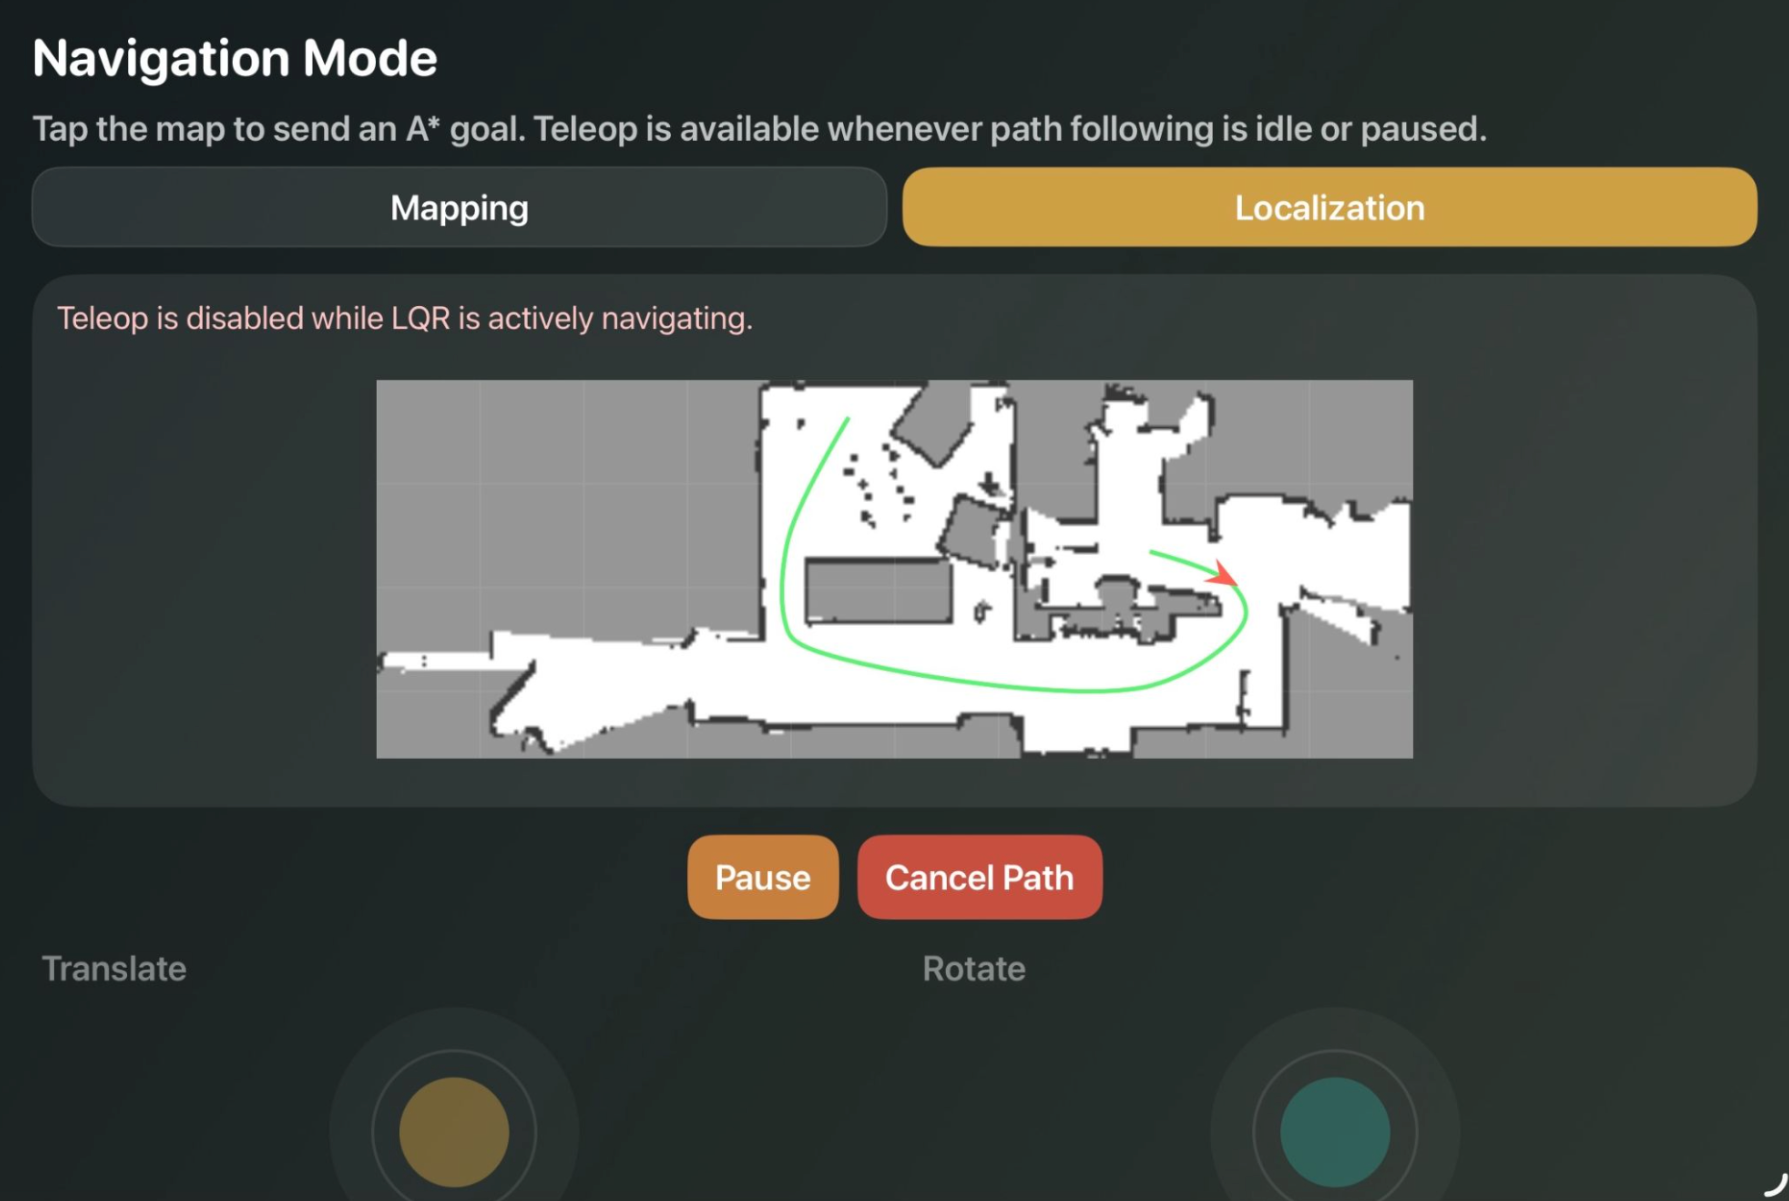
\includegraphics[width=0.56\textwidth]{mobile.png}
    \caption{Paesano mobile application interface for telemetry, teleoperation, and navigation control. The screenshot shows the navigation mode, including live map display, goal selection, and path visualization.}
    \label{fig:paesano-mobile-app}
\end{figure}

\section{Experiments}
To evaluate Paesano at both the low-level control and high-level autonomy levels, two experiments were conducted. The first isolates drivetrain command tracking and stop behavior. The second evaluates the full autonomy stack by measuring how closely the robot follows planned trajectories in the map frame. Together, these experiments validate the platform from motor control through navigation execution.
\subsection{Velocity and Position Control Performance}
For the low-level velocity and position control tests, ROS 2 bags were recorded
while forward, lateral, and rotational commands were applied over multiple
different magnitudes. The bags included \texttt{/cmd\_vel}, \texttt{/odom},
\texttt{/odom/filtered}, and \texttt{/wheel\_encoders}. From these logs, rise
behavior, overshoot, settling, and residual stop error were observed. When a
historical test bag contained a command larger than the final enforced
controller limit, the analysis treated that command as the corresponding
effective cap of \SI{0.35}{m/s} for translation or \SI{1.5}{rad/s} for
rotation.

\begin{table}[H]
    \centering
    \caption{Average low-level control metrics across the recorded velocity-control trials.}
    \label{tab:velocity-control-summary}
    \small
    \begin{tabular}{lcccc}
        \toprule
        Motion & \shortstack{Mean steady-state\\error} & Mean overshoot & \shortstack{Mean stop\\decay} & \shortstack{Mean encoder\\stop error} \\
        \midrule
        Forward & \SI{-0.0067}{m/s} & \SI{5.79}{\percent} & \SI{0.35}{s} & \SI{0.0097}{m} \\
        Lateral & \SI{-0.0056}{m/s} & \SI{5.66}{\percent} & \SI{0.25}{s} & \SI{0.0073}{m} \\
        Rotation & \SI{-0.0245}{rad/s} & \SI{11.06}{\percent} & \SI{0.33}{s} & N/A \\
        \bottomrule
    \end{tabular}
\end{table}

\noindent The forward and lateral responses were consistent across trials,
with small overshoot and short residual settling after the command returned to
zero. Forward tracking was the cleanest overall, with a mean steady-state error
of \SI{-0.0067}{m/s}, indicating that the measured forward speed settled only
slightly above the effective command. Lateral motion remained similarly well
controlled, with a mean steady-state error of \SI{-0.0056}{m/s}, although its
stop-position behavior still reflected the higher slip sensitivity of mecanum
strafing. Rotational tracking also settled quickly, with a mean steady-state
error of \SI{-0.0245}{rad/s}. This negative sign again indicates mild
overtracking rather than underspeed. Even so, the post-stop rotational decay
remained short and consistent, which is the more important behavior for the
higher-level navigation stack.

\begin{figure}[H]
    \centering
    \begin{subfigure}{0.49\textwidth}
        \centering
        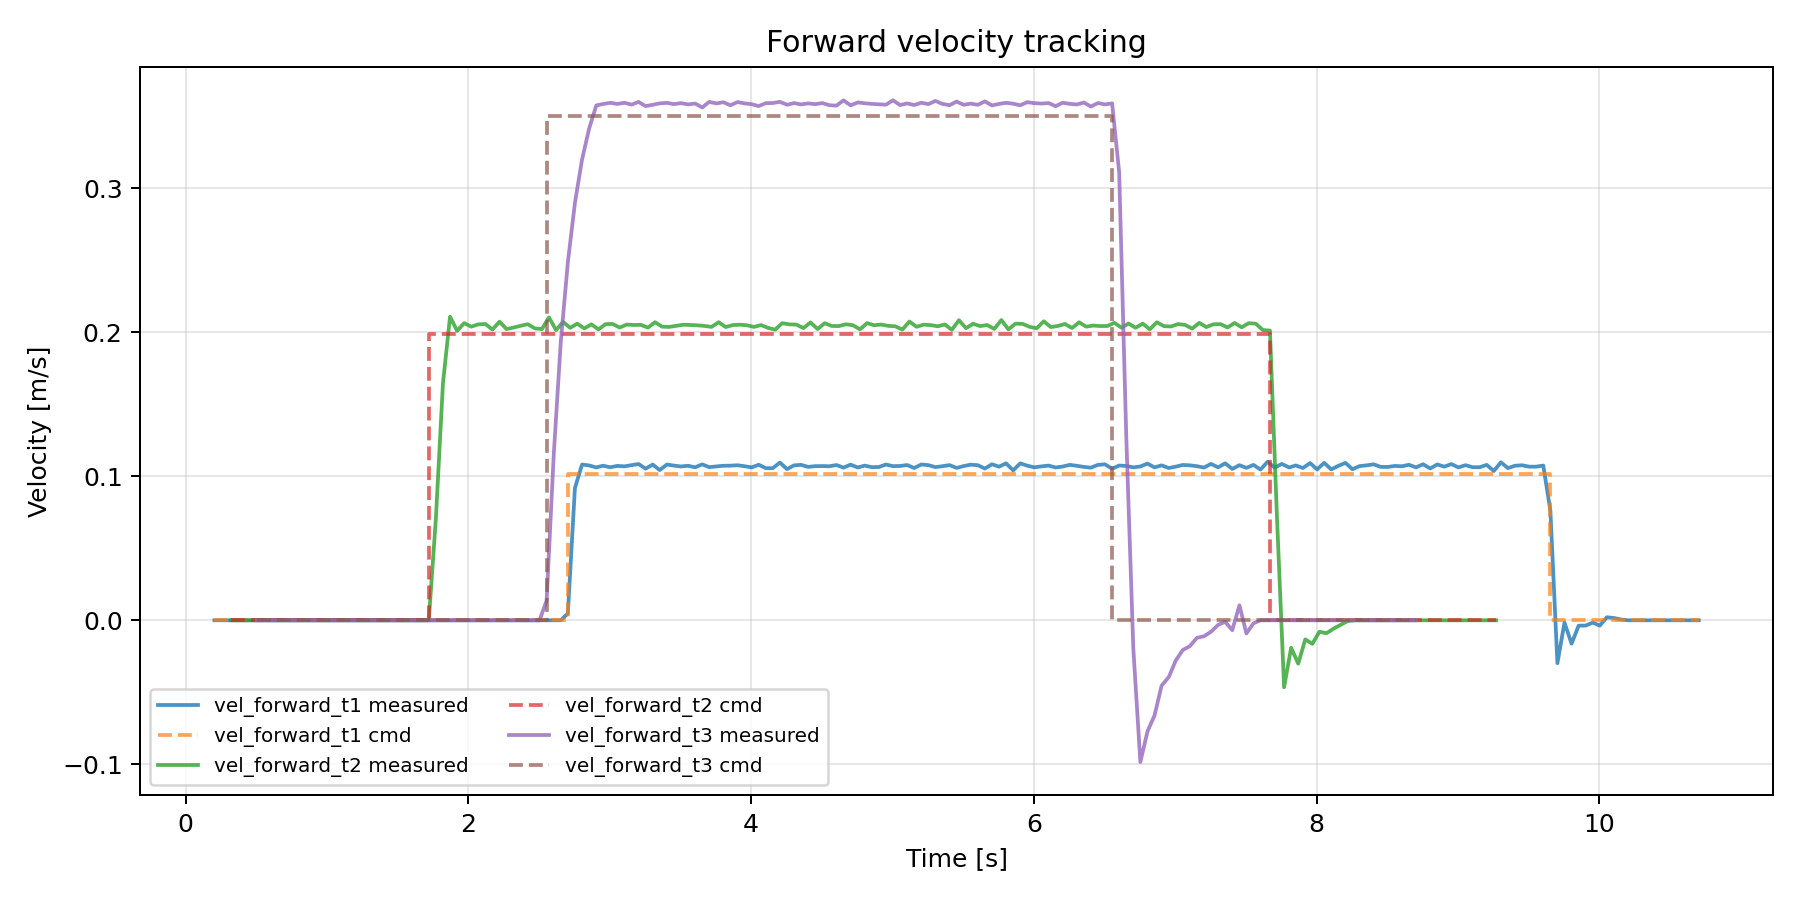
\includegraphics[width=\linewidth]{experiments/forward_overlay.png}
        \caption{Forward velocity tracking.}
        \label{fig:forward-overlay}
    \end{subfigure}
    \hfill
    \begin{subfigure}{0.49\textwidth}
        \centering
        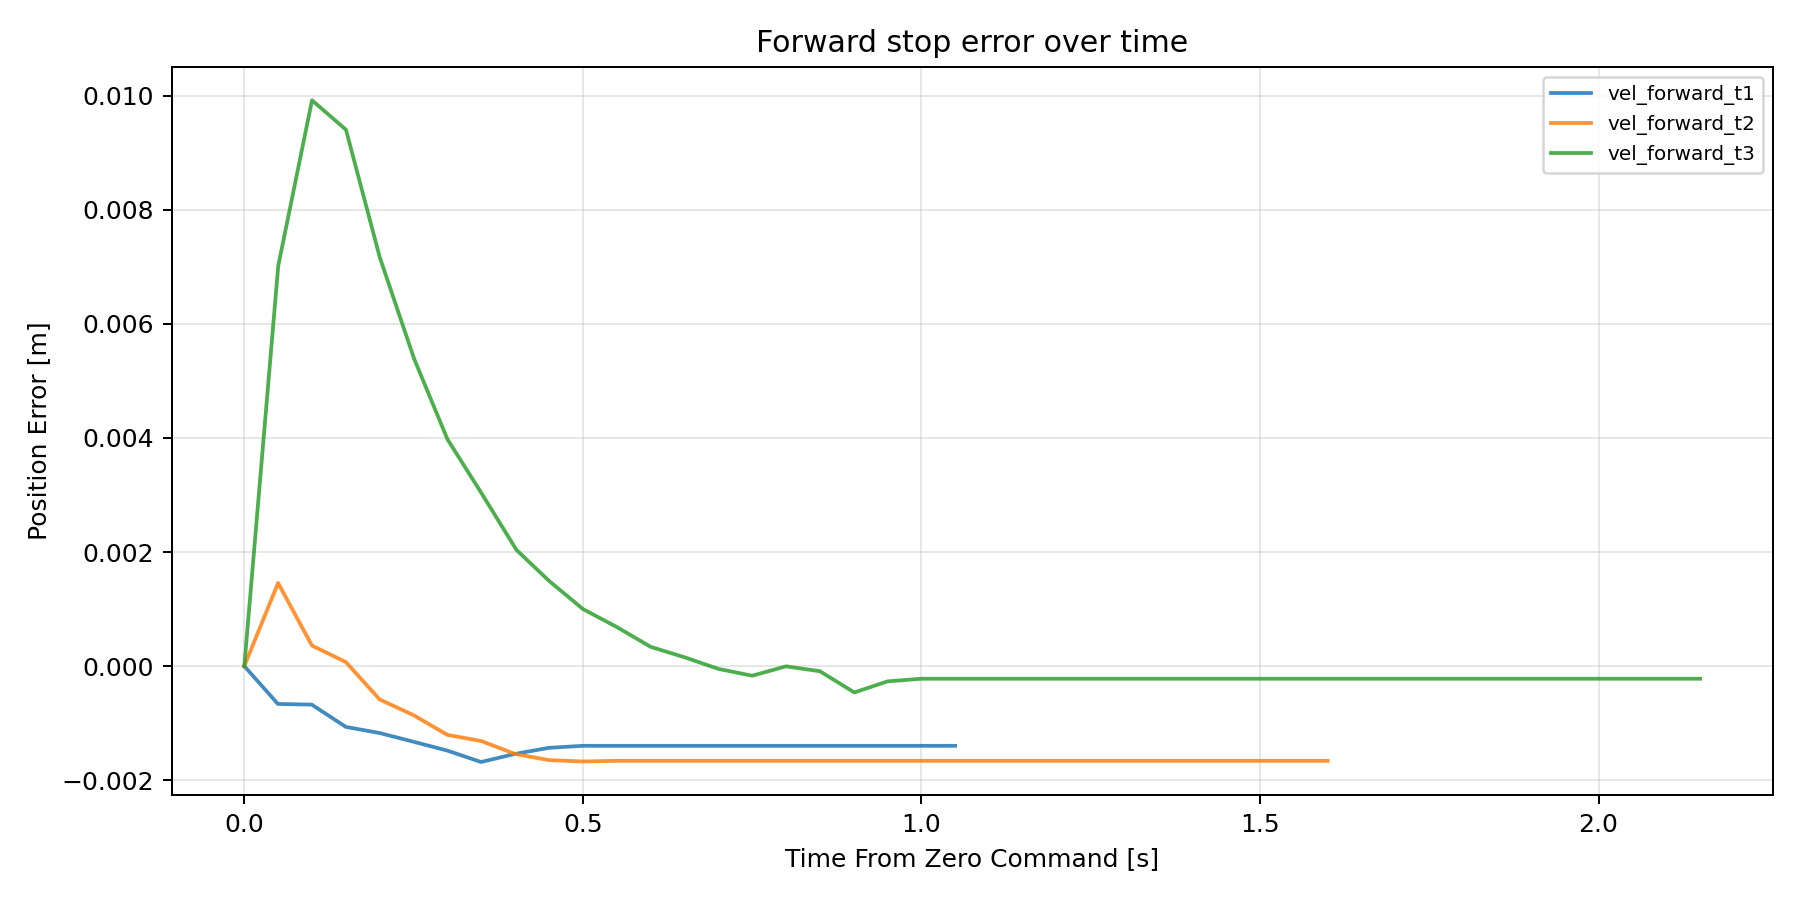
\includegraphics[width=\linewidth]{experiments/forward_stop_error_time.png}
        \caption{Forward stop error after zero command.}
        \label{fig:forward-stop-error}
    \end{subfigure}
    \caption{Forward-axis low-level control performance. The measured response closely tracks the commanded input, with only a brief braking transient when the command returns to zero.}
    \label{fig:forward-control-results}
\end{figure}

\begin{figure}[H]
    \centering
    \begin{subfigure}{0.49\textwidth}
        \centering
        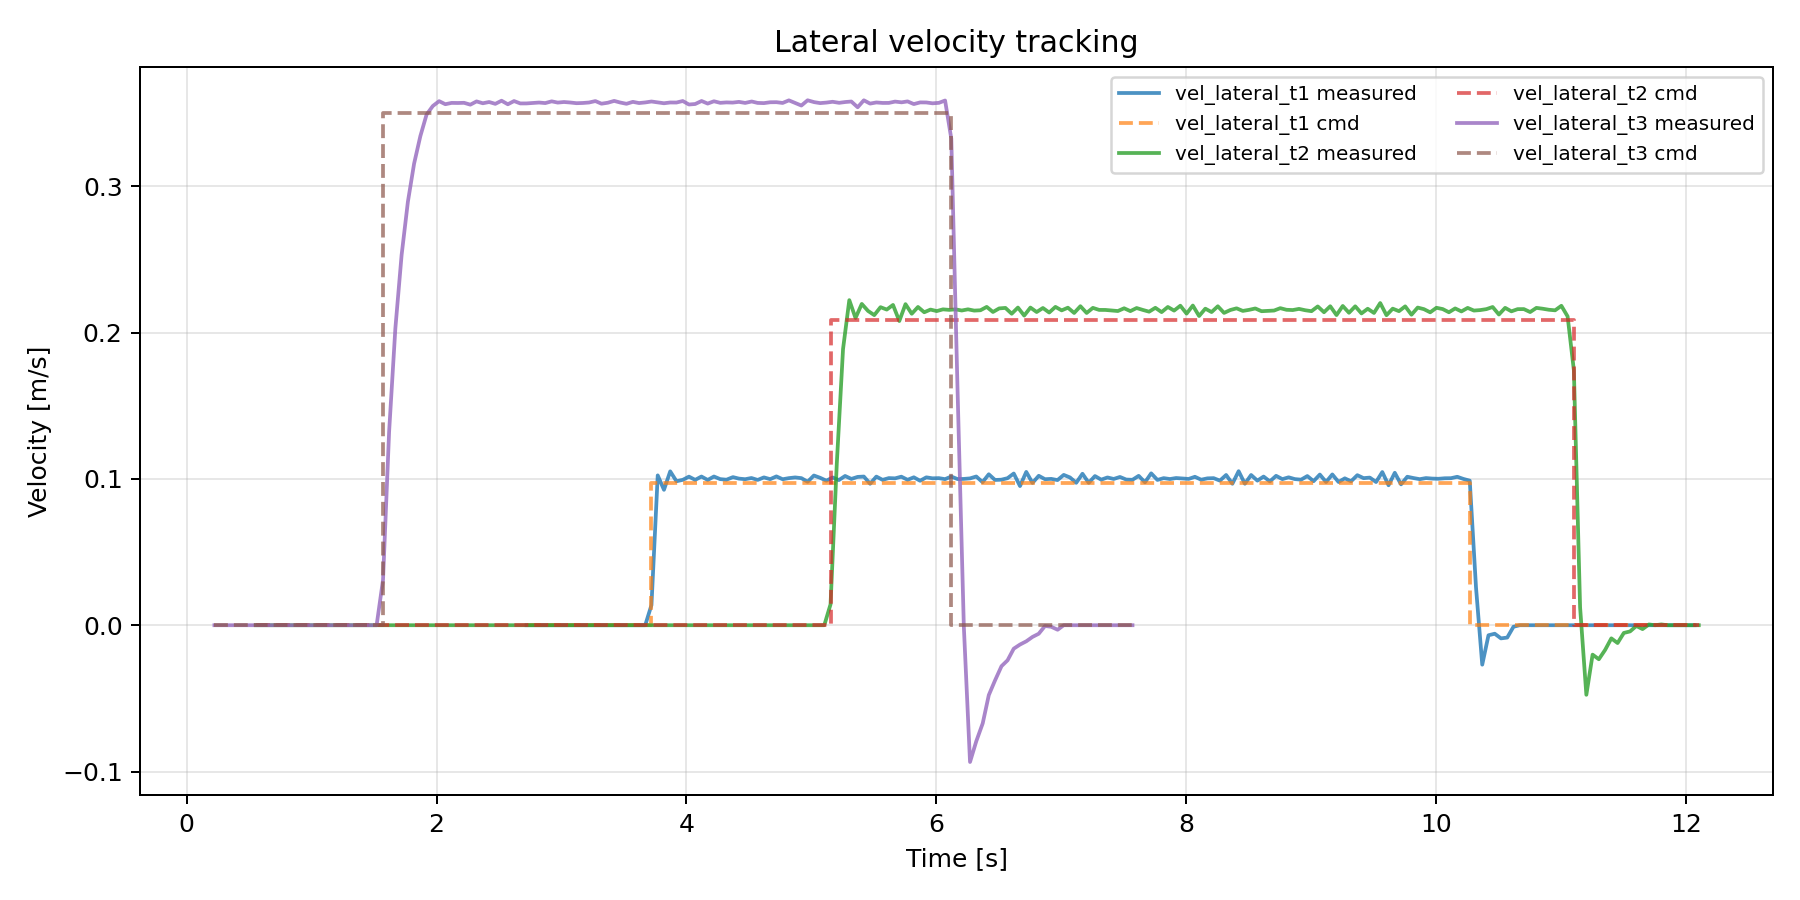
\includegraphics[width=\linewidth]{experiments/lateral_overlay.png}
        \caption{Lateral velocity tracking.}
        \label{fig:lateral-overlay}
    \end{subfigure}
    \hfill
    \begin{subfigure}{0.49\textwidth}
        \centering
        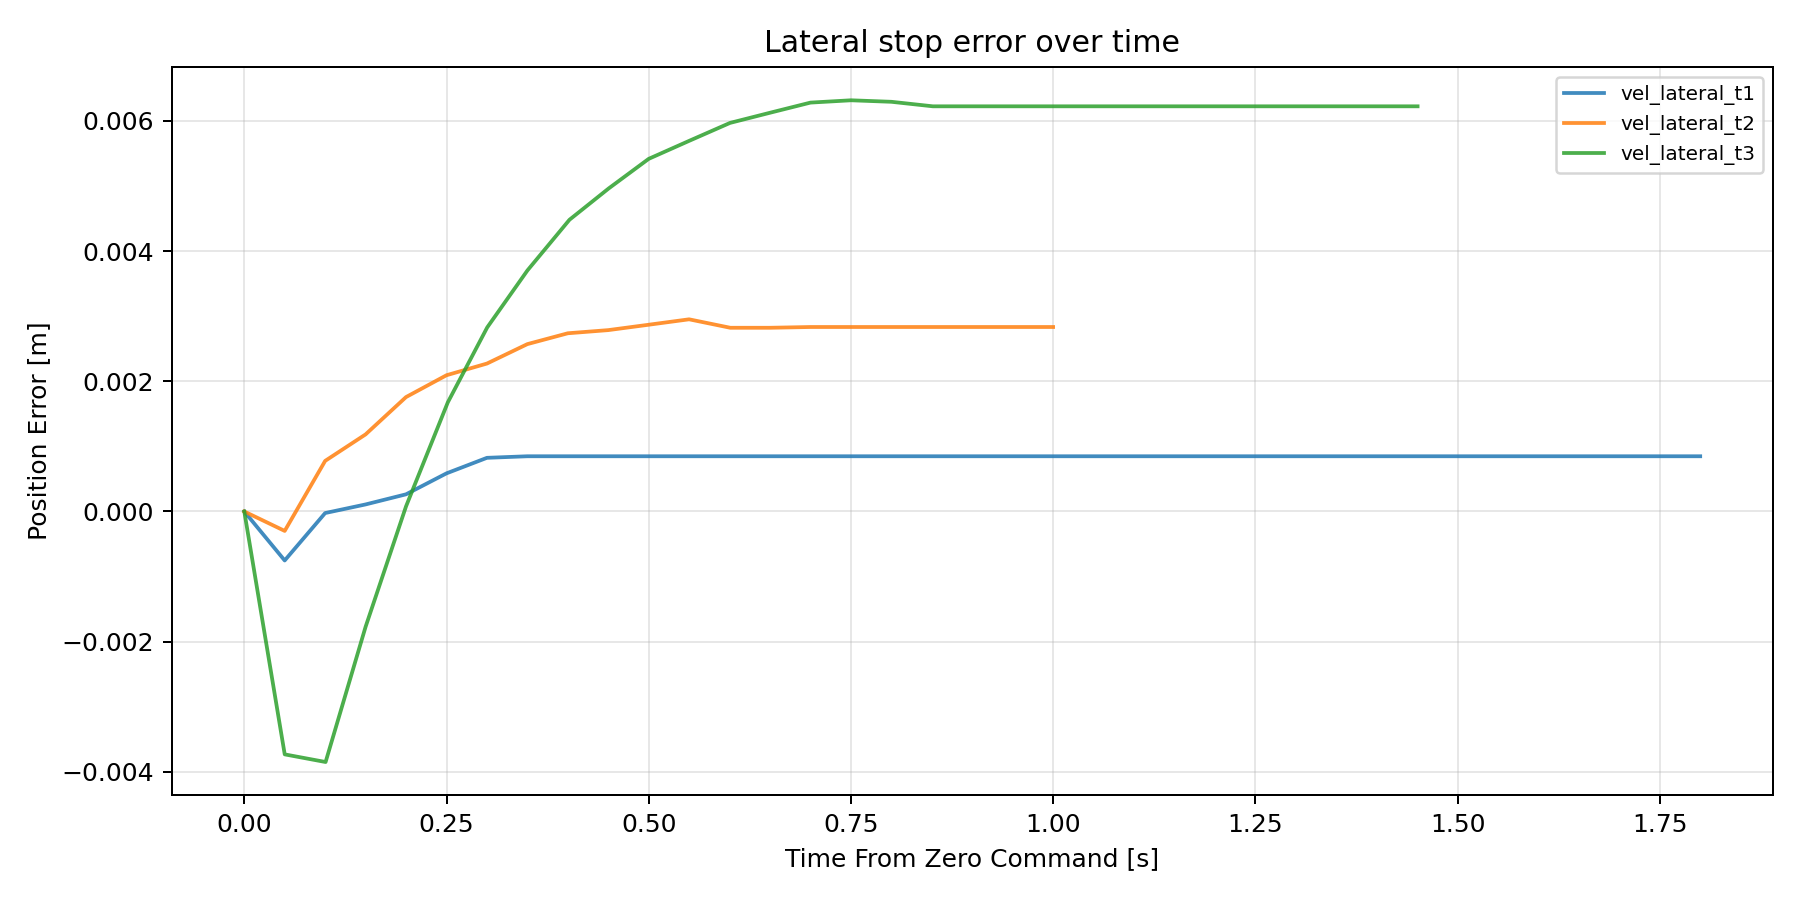
\includegraphics[width=\linewidth]{experiments/lateral_stop_error_time.png}
        \caption{Lateral stop error after zero command.}
        \label{fig:lateral-stop-error}
    \end{subfigure}
    \caption{Lateral-axis low-level control performance. Strafing remained stable and repeatable, although slightly less precise than the forward axis.}
    \label{fig:lateral-control-results}
\end{figure}

\begin{figure}[H]
    \centering
    \begin{subfigure}{0.49\textwidth}
        \centering
        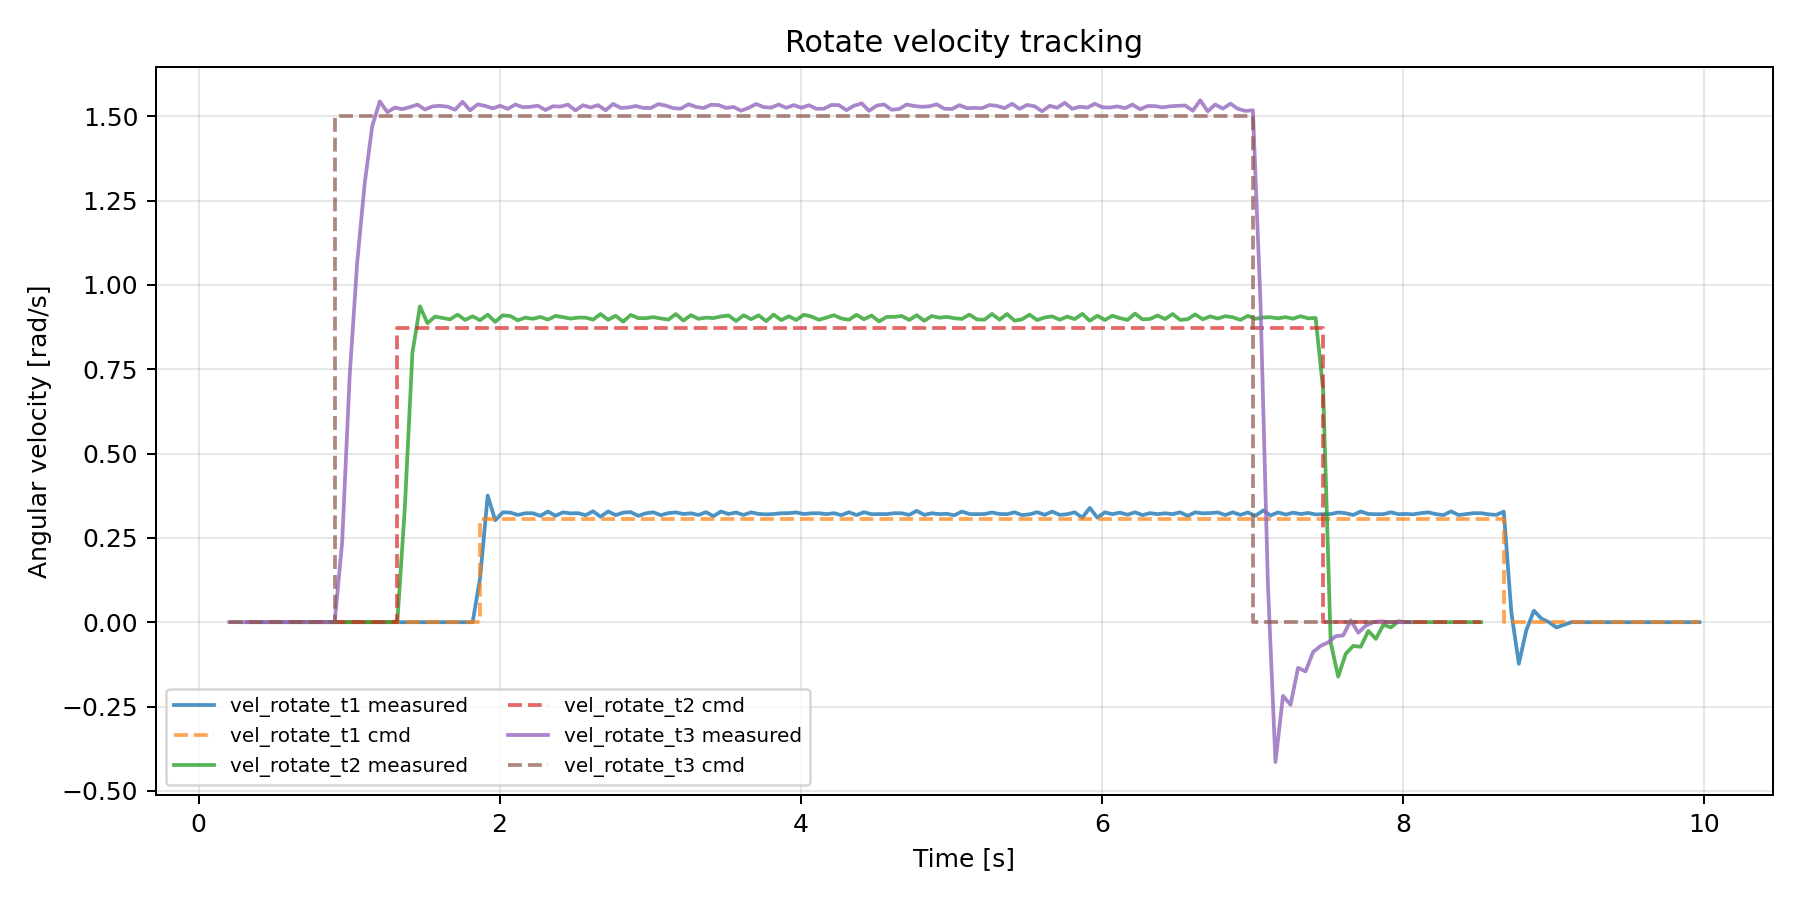
\includegraphics[width=\linewidth]{experiments/rotate_overlay.png}
        \caption{Angular velocity tracking.}
        \label{fig:rotate-overlay}
    \end{subfigure}
    \hfill
    \begin{subfigure}{0.49\textwidth}
        \centering
        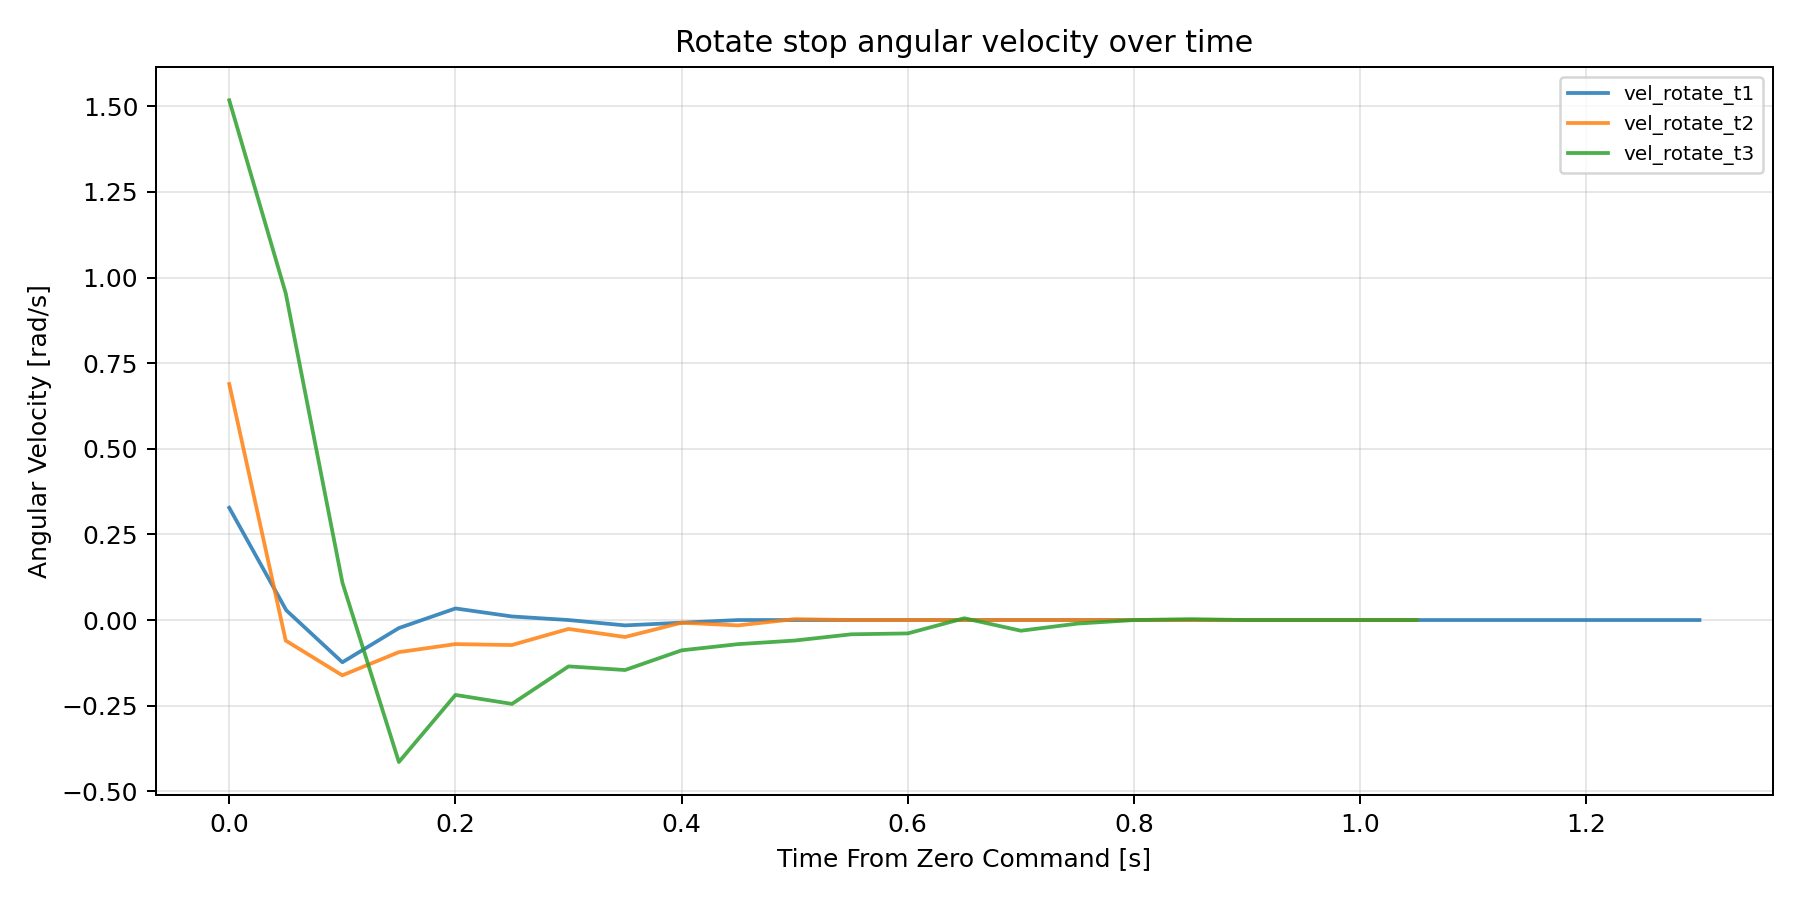
\includegraphics[width=\linewidth]{experiments/rotate_stop_velocity_time.png}
        \caption{Angular velocity decay after zero command.}
        \label{fig:rotate-stop-error}
    \end{subfigure}
    \caption{Rotational low-level control performance. The turn response exhibits slightly higher transient error at large commands, but the stop behavior remains sharp and repeatable.}
    \label{fig:rotation-control-results}
\end{figure}

\subsection{Trajectory Following Performance}
\noindent The second experiment evaluated the full autonomy stack in localization
mode. Three routes were tested: a straight route, a single-turn curve route, and
a longer multi-segment route through a more cluttered portion of the map. Each
route was executed three times from a fixed marked start pose, and ROS 2 bags
were recorded containing \texttt{/path}, \texttt{/estimated\_pose},
\texttt{/odom/filtered}, \texttt{/cmd\_vel}, and \texttt{/map}. The primary
metrics were completion time, final position error, final heading error, and
cross-track error with respect to the planned path.

\noindent This experiment intentionally validates more than just the tracking
controller. Because the robot is operating in the map frame while using the full
navigation stack, the results reflect the combined behavior of localization,
global planning, path pruning, spline generation, and LQR tracking. Route-following accuracy therefore also captures localization quality implicitly, since the pose estimator must remain consistent over the full run for the robot to remain on the planned path.

\begin{table}[H]
    \centering
    \caption{Average trajectory-following results by route type.}
    \label{tab:trajectory-summary}
    \small
    \begin{tabular}{lccccc}
        \toprule
        Route & \shortstack{Mean completion\\time} & \shortstack{Mean final\\position error} & \shortstack{Mean cross-track\\error} & \shortstack{Mean final\\heading error} & Success \\
        \midrule
        Straight & \SI{6.11}{s} & \SI{0.0041}{m} & \SI{0.0089}{m} & \SI{0.154}{deg} & 3/3 \\
        Curve & \SI{18.29}{s} & \SI{0.0041}{m} & \SI{0.0086}{m} & \SI{0.366}{deg} & 3/3 \\
        Complex & \SI{44.09}{s} & \SI{0.0095}{m} & \SI{0.0087}{m} & \SI{0.270}{deg} & 3/3 \\
        \bottomrule
    \end{tabular}
\end{table}

\noindent Across all nine recorded navigation runs, the mean cross-track error in
the LiDAR-localized map frame was \SI{0.0088}{m}, the mean final position error
was \SI{0.0059}{m}, and every trial completed successfully. These values are
strong for a student-built indoor mobile platform and indicate that the path
planner, spline generator, and LQR tracker are all operating consistently in
the same frame as the localization estimate. Because the metric is computed
from the estimated pose and planned path in the map frame rather than from an
external ground-truth system, it should be interpreted as estimated
route-following accuracy relative to the LiDAR-based localization solution. The
straight route produced the smallest directional variation, while the curve and
complex routes remained nearly identical in mean cross-track error despite the
larger path length and longer execution time.

\begin{figure}[H]
    \centering
    \begin{subfigure}{0.49\textwidth}
        \centering
        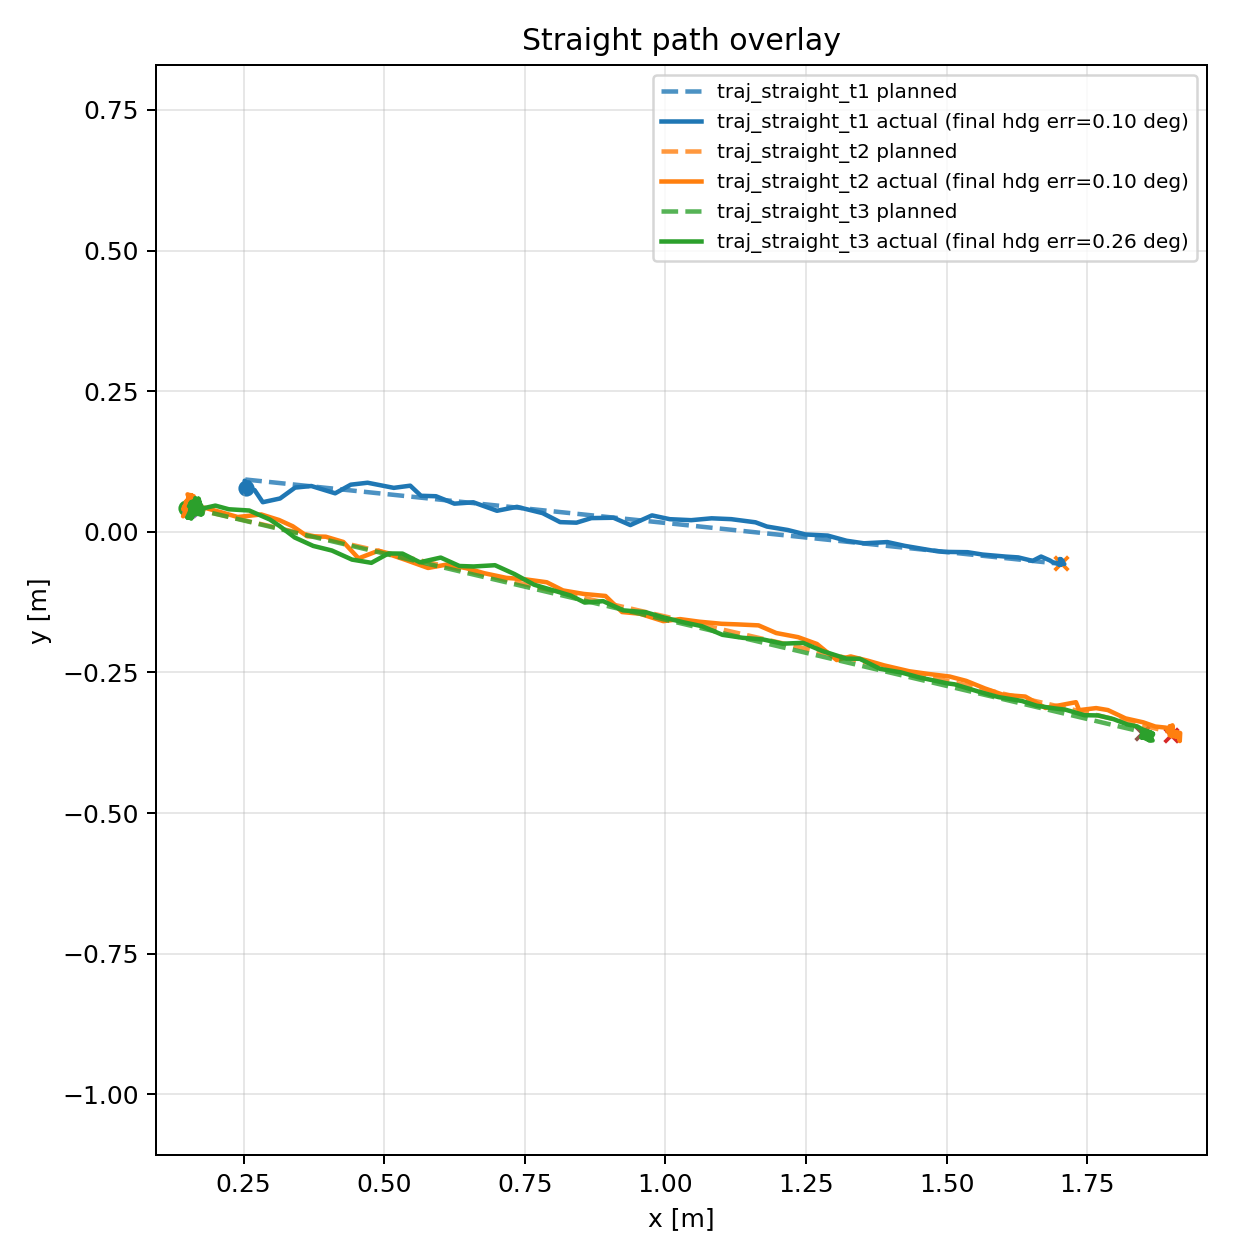
\includegraphics[width=\linewidth]{experiments/straight_overlay.png}
        \caption{Straight-route planned and actual paths.}
        \label{fig:straight-overlay}
    \end{subfigure}
    \hfill
    \begin{subfigure}{0.49\textwidth}
        \centering
        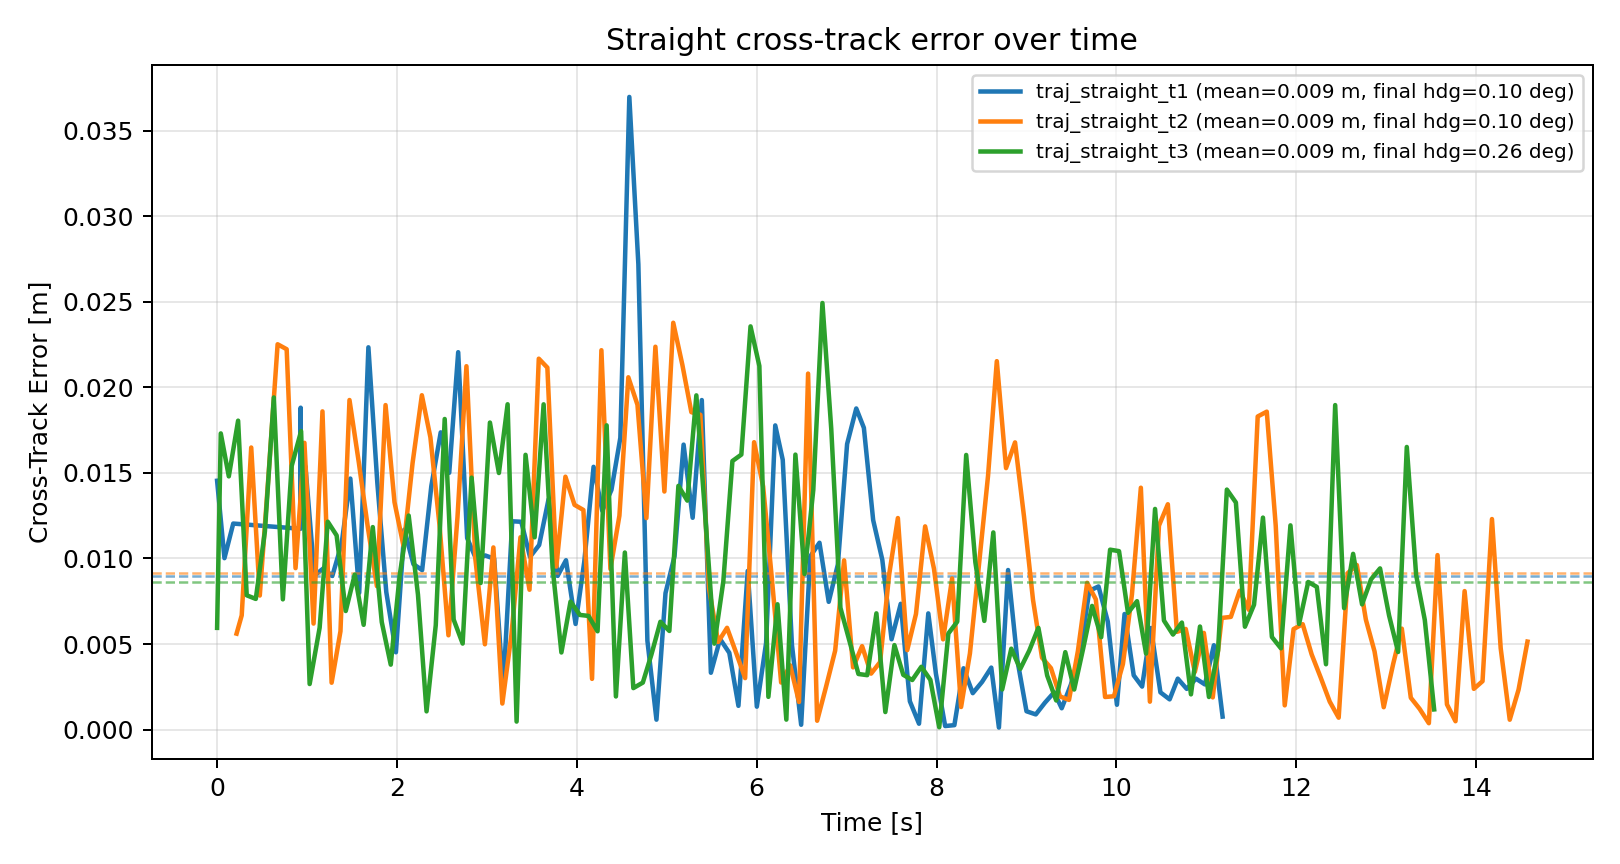
\includegraphics[width=\linewidth]{experiments/straight_cross_track_error.png}
        \caption{Straight-route cross-track error over time.}
        \label{fig:straight-cross-track}
    \end{subfigure}
    \caption{Trajectory-following results for the straight route. The actual path remains nearly coincident with the planned reference, and the cross-track error stays small throughout the run.}
    \label{fig:straight-route-results}
\end{figure}

\begin{figure}[H]
    \centering
    \begin{subfigure}{0.49\textwidth}
        \centering
        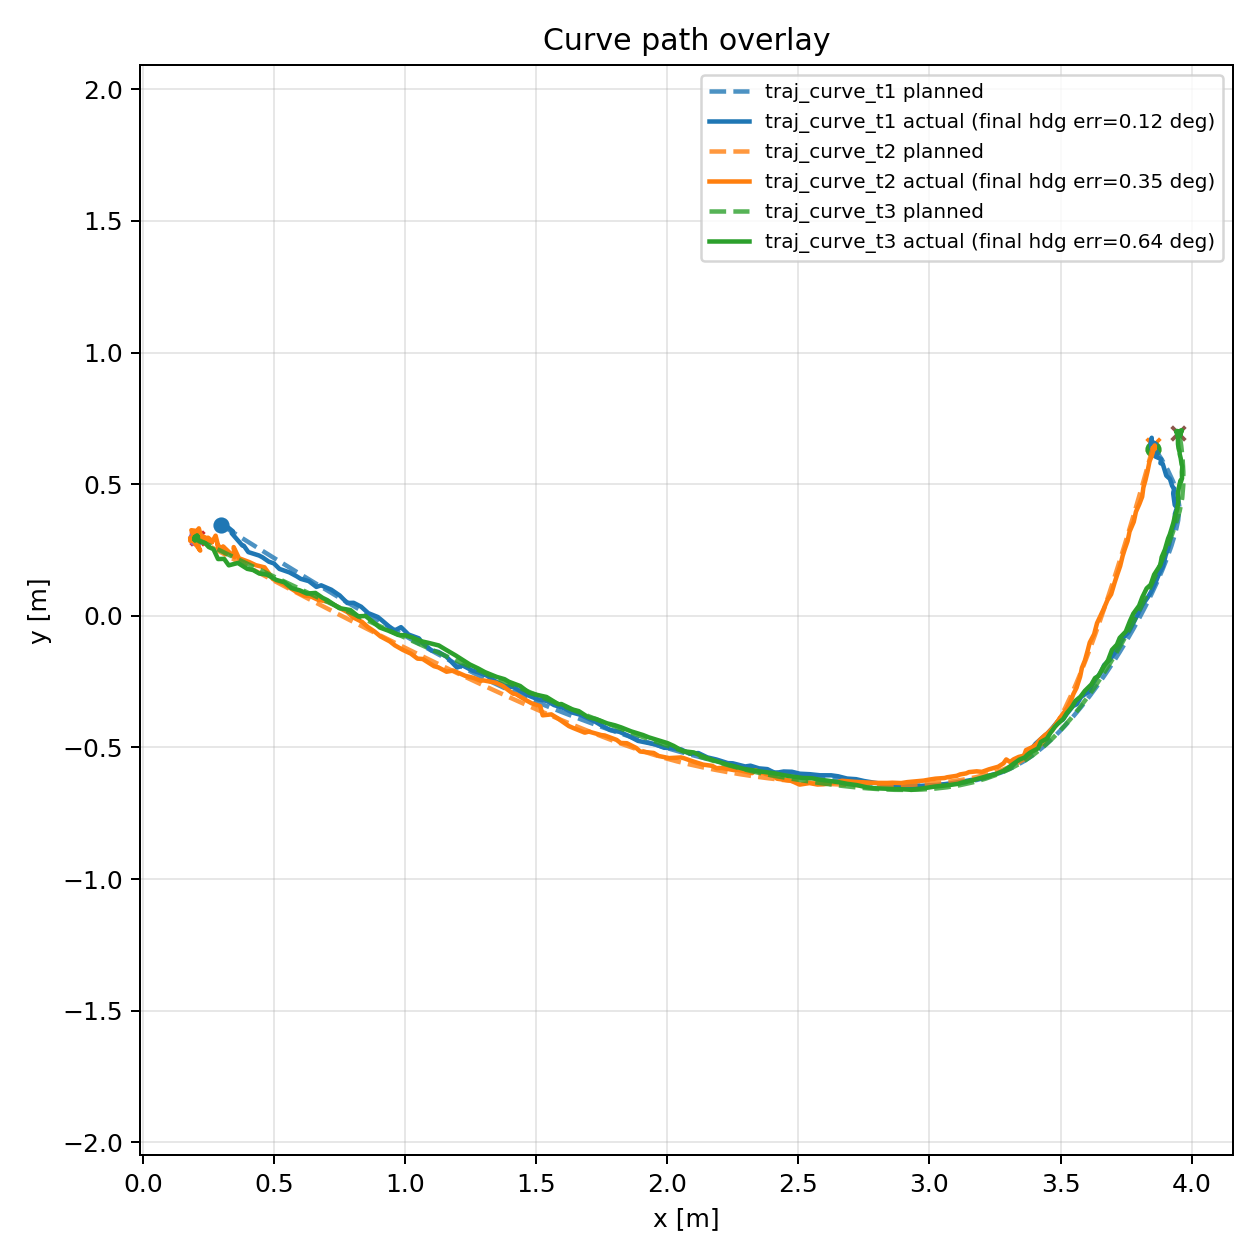
\includegraphics[width=\linewidth]{experiments/curve_overlay.png}
        \caption{Curve-route planned and actual paths.}
        \label{fig:curve-overlay}
    \end{subfigure}
    \hfill
    \begin{subfigure}{0.49\textwidth}
        \centering
        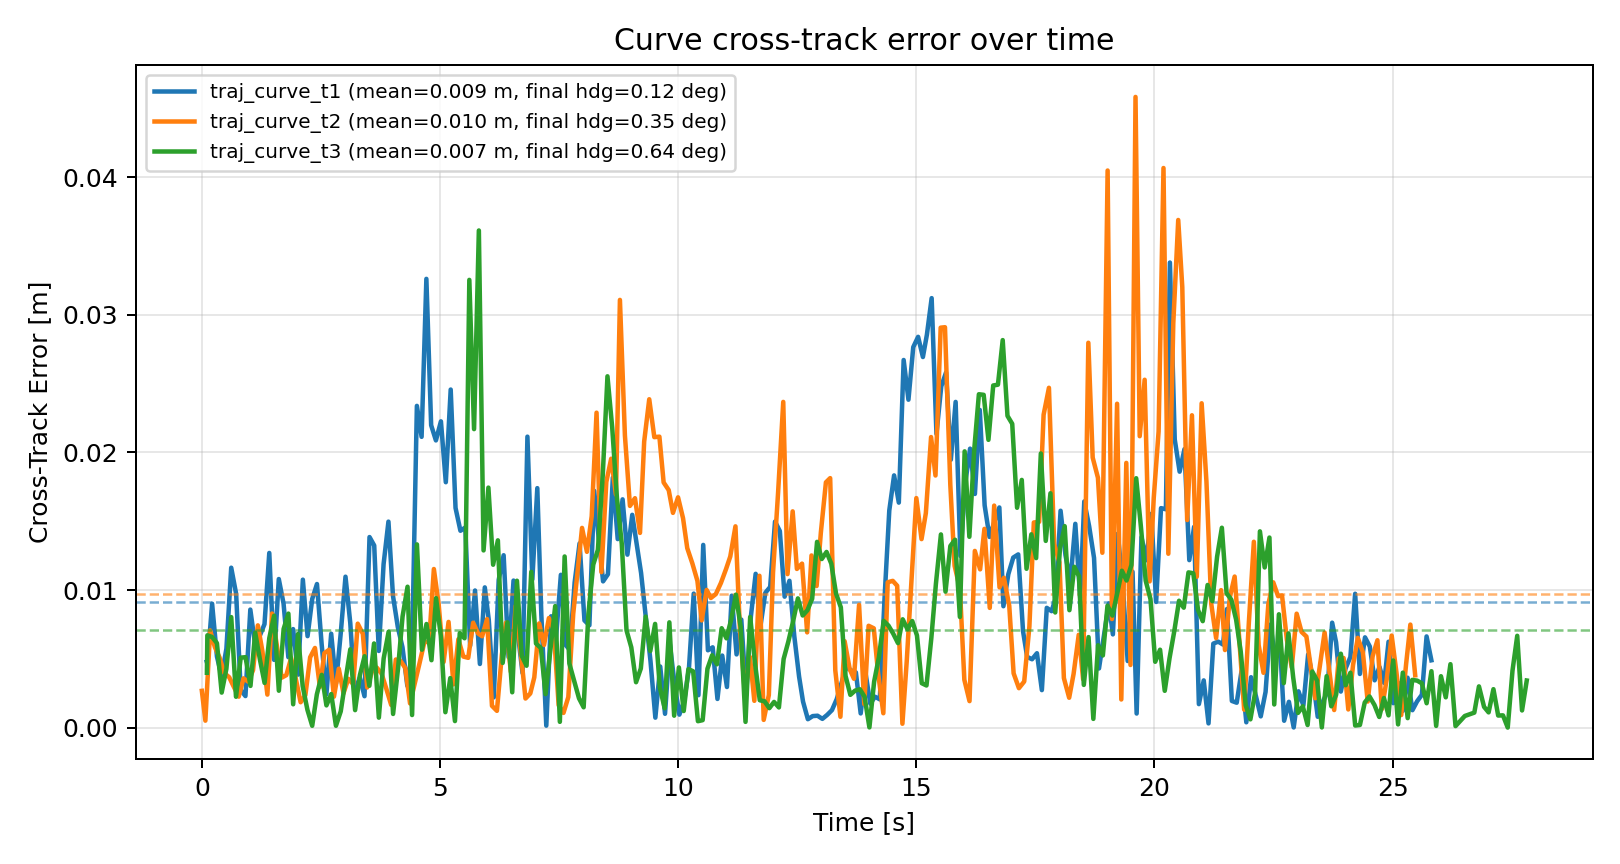
\includegraphics[width=\linewidth]{experiments/curve_cross_track_error.png}
        \caption{Curve-route cross-track error over time.}
        \label{fig:curve-cross-track}
    \end{subfigure}
    \caption{Trajectory-following results for the single-turn curve route. The controller remains tightly aligned with the planned reference through the turn.}
    \label{fig:curve-route-results}
\end{figure}

\begin{figure}[H]
    \centering
    \begin{subfigure}{0.49\textwidth}
        \centering
        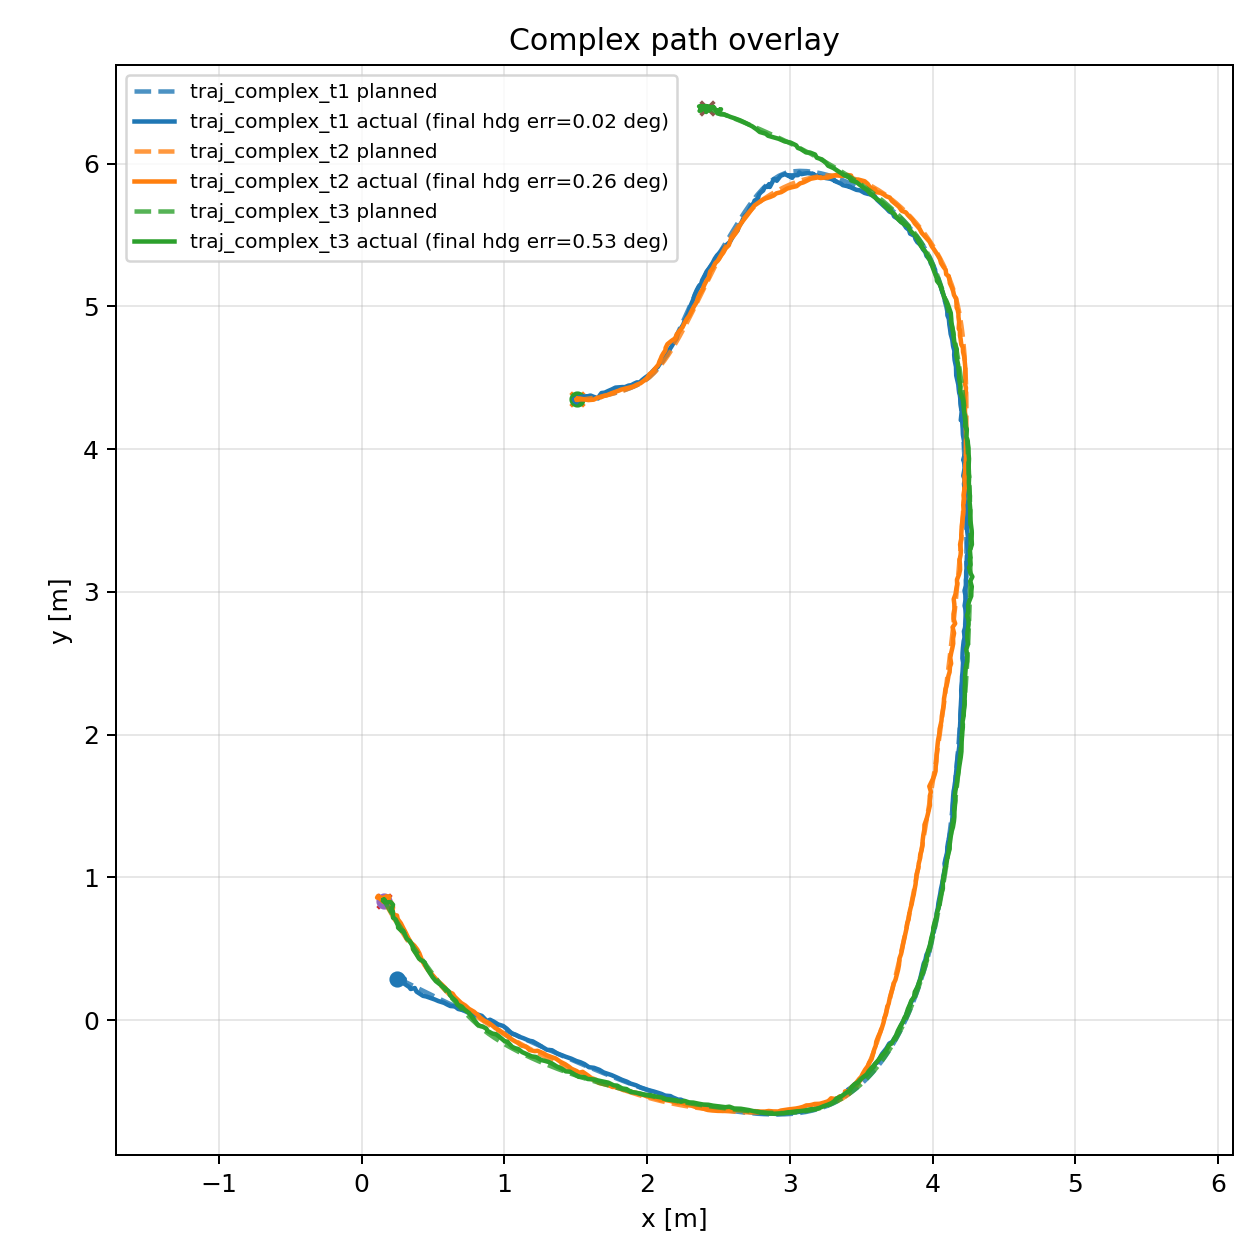
\includegraphics[width=\linewidth]{experiments/complex_overlay.png}
        \caption{Complex-route planned and actual paths.}
        \label{fig:complex-overlay}
    \end{subfigure}
    \hfill
    \begin{subfigure}{0.49\textwidth}
        \centering
        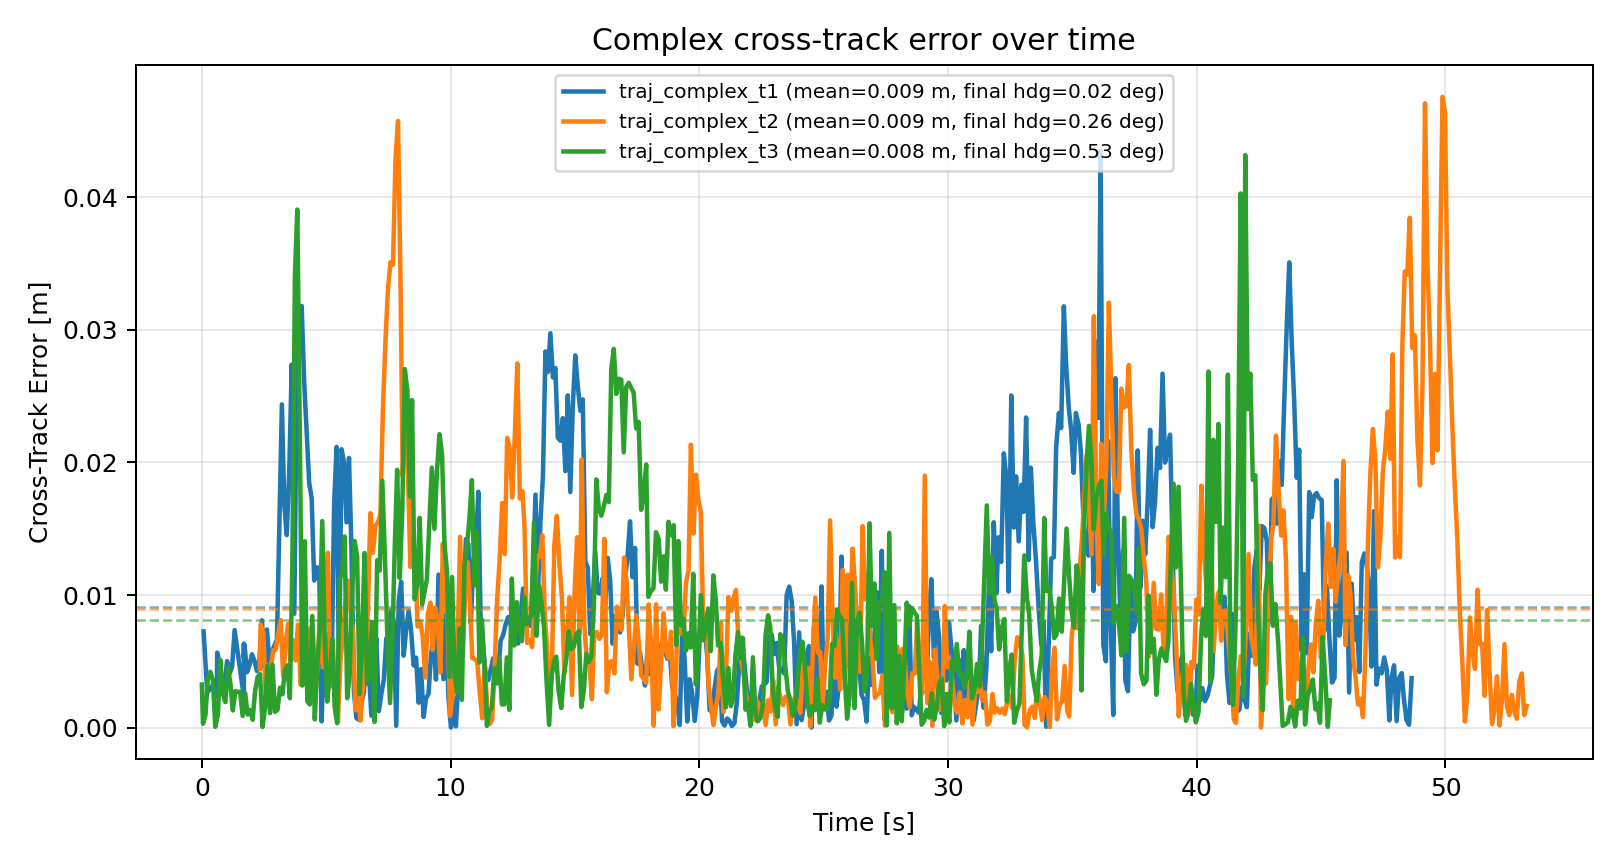
\includegraphics[width=\linewidth]{experiments/complex_cross_track_error.png}
        \caption{Complex-route cross-track error over time.}
        \label{fig:complex-cross-track}
    \end{subfigure}
    \caption{Trajectory-following results for the complex multi-segment route. Even on the longest path, the measured tracking error remains small relative to the map scale.}
    \label{fig:complex-route-results}
\end{figure}

\section{Conclusion and Future Improvements}
Paesano was a successful implementation of a holonomic indoor autonomous mobile robot, integrating embedded motor control, state estimation, localization, mapping, global planning, and trajectory following.
Some of the highlights of this project include:
\begin{itemize}
    \item Low-level control was stable and repeatable with an average steady-state error of -0.0067m/s in the forward axis, -0.0056m/s in the lateral axis, and -0.0245rad/s in rotation.
    \item The autonomous navigation stack produced accurate trajectory following with a mean cross-track error of 0.0088m, final position error of 0.0059m, and a mean final heading error of 0.263 degrees across all trials, demonstrating the effectiveness of the EKF, MCL, A$^{*}$ planner, and LQR controller working together in the map frame.
    \item The mobile application provided a user-friendly interface for teleoperation, map visualization, and navigation control, effectively bridging the autonomy stack and human operator.
\end{itemize}
These results validate the core system works together seamlessly, as estimation, planning, and control all have to be consistent for the robot to follow the path so accurately. However, 
it is important to acknowledge that these results were measured in the map frame, not external ground truth. Therefore, the reported errors reflect the internal consistency of the autonomy stack rather than absolute accuracy in the physical environment.
Given the complexity of the system and the fact that it was built from scratch, these results are strong and demonstrate that the core algorithms and hardware design are sound. The robot is able to navigate through the environment while maintaining a tight trajectory relative to its internal map and localization estimate
and if ground truth were available, the absolute errors may differ.
Some current limitations and areas for future improvement include:
\begin{itemize}
    \item Dynamic Obstacle Avoidance: The current planner does not account for dynamic obstacles, which could lead to collisions in environments with moving people or objects. Future work could integrate a local obstacle avoidance layer that reacts to real-time sensor data while following the global path.
    \item Semantic Control: The current control strategy is purely geometric and is not aware of the semantic context of the environment. Future improvements could include higher-level reasoning about room types, doorways, or human presence to implement features such as "wait at the door", "avoid crowded areas", or "follow me" behaviors.
    \item Ground Truth Evaluation: The current experiments rely on the internal map frame for error metrics. Future work could incorporate an external motion capture system or visual odometry to provide absolute ground truth measurements of localization and trajectory-following accuracy.
\end{itemize}

\end{document}
